\section{Gauge representatives and their physical meaning}
\label{app:theory}
This appendix develops the \hyperref[app:vector-gauge]{gauge projection}, \hyperref[app:spectrum]{spectral correspondence}, and \hyperref[app:topology-rom]{harmonic completion} used in the construction. \hyperref[app:protocol]{Experimental protocols}, \hyperref[app:3d-controls]{three-dimensional comparisons}, \hyperref[app:fields]{flow visualizations}, and \hyperref[app:modes]{mode atlases} follow the mathematical details.

\subsection{Scalar constants and boundary-pinned representatives}
\label{app:scalar}
For a connected domain, $\nabla^\perp(\psi+c)=\nabla^\perp\psi$. The mean-zero projection $P_0\psi=\psi-\langle\psi\rangle_\Omega$ is invariant to a constant shift, preserves all spatial derivatives, and selects a unique representative. Let $w$ be the column vector of positive quadrature weights, $\mathbf1$ the all-ones vector, and $\psi_q=\psi(\mathbf x_q)$. The discrete projector is $P_0=I-\mathbf1 w^{\top}/(\mathbf1^{\top}w)$; backpropagation uses its transpose in Euclidean coordinates. In particular,
\[
\sum_q w_q(P_0\psi)_q=0,\qquad
\norm{P_0\psi}_Q^2=\norm{\psi}_Q^2-\frac{(\sum_qw_q\psi_q)^2}{\sum_qw_q}.
\]
For a periodic scalar potential, this removes the constant kernel before the spectral mass is formed. Without removal, $\norm{\nabla(\psi+c)}^2/\norm{\psi+c}^2\to0$ as $|c|\to\infty$, although the physical velocity is unchanged.

For a homogeneous Dirichlet scalar eigenproblem, $\psi=0$ on the boundary excludes nonzero constant shifts from the admissible space and fixes the representative used in its mass form. Centering this function changes the mass form and is therefore used here for display only: it changes the common boundary value to $-\langle\psi\rangle_\Omega$ while preserving velocity. Finite-element scalar displays use area-weighted means, and periodic displays use uniform-grid means.

On a multiply connected domain, independent boundary constants encode physical harmonic velocities. Subtracting one global constant preserves their differences. It therefore fixes scalar gauge without deleting circulation degrees of freedom. Each connected component requires its own additive convention if the fluid domain itself is disconnected.

\subsection{Vector gauge as a quotient-space projection}
\label{app:vector-gauge}
Let $d_R^k$ denote exterior differentiation of degree-$k$ forms with relative boundary trace; its adjoint is $\delta_R^{k+1}$. The closed potential-to-velocity operator is $\C=\star d_R^{D-2}$. Writing $\ker$ for the nullspace and $\perp$ for mass-orthogonal complement, the canonical potential space is $(\ker\C)^\perp$. In 3D, exact-gradient removal is the orthogonal projection defined using scalar test functions $\eta\in H_0^1(\Omega)$, where $H_0^1$ is the Sobolev space of functions with square-integrable first derivatives and zero boundary trace:
\[
\ip{\nabla\phi}{\nabla\eta}=\ip{\widetilde{\mathbf A}}{\nabla\eta},\qquad \eta\in H_0^1(\Omega).
\]
Integration by parts gives \doceqref{eq:poisson-gauge}. Removing the remaining relative harmonic kernel completes the projection. Both corrections have zero curl, and a Dirichlet scalar has no tangential derivative on the boundary, so curl and the relative tangential trace are preserved.

To see why this operation belongs before the loss, choose a nonzero $\kappa\in\ker\C$. The family $\mu_\alpha=\mu+\alpha\kappa$ represents exactly the same velocity for every real scalar $\alpha$, yet
\begin{equation}
\frac{\norm{\C\mu_\alpha}^2}{\norm{\mu_\alpha}^2}
=\frac{\norm{\C\mu}^2}{\norm{\mu+\alpha\kappa}^2}\longrightarrow0
\quad\text{as }|\alpha|\longrightarrow\infty.
\end{equation}
The unprojected quotient can therefore decrease without improving a physical mode. On the canonical space this ambiguity disappears. Write $L^2\Lambda^k$ for square-integrable degree-$k$ forms, $\operatorname{Ran}$ for operator range, an overline for closure, and $\oplus$ for orthogonal direct sum. The relative harmonic space $\Harm_R^k$ contains the closed, coclosed forms with relative boundary trace. With the orthogonal Hodge decomposition {\citep{arnold2006finite}}
\begin{equation}
L^2\Lambda^{D-2}=\overline{\operatorname{Ran}d_R^{D-3}}
\oplus\Harm_R^{D-2}\oplus\overline{\operatorname{Ran}\delta_R^{D-1}},
\end{equation}
the last summand is $(\ker\C)^\perp$. Let $\Delta_H=d\delta+\delta d$ be the positive Hodge Laplacian and $G_R$ its relative-boundary Green pseudoinverse. The exact projector is $P_{\rm gf}=\delta_R d_R G_R$, and it satisfies
\begin{equation}
P_{\rm gf}(\mu+\kappa)=P_{\rm gf}\mu,\quad
\C P_{\rm gf}\mu=\C\mu,\quad
\delta_R P_{\rm gf}\mu=0.
\end{equation}
Normalization and Gram--Schmidt consequently act on physical equivalence classes. In a finite auxiliary space, the invariance identity applies to the resolved kernel directions; \docref{Appendix}{app:3d-controls} quantifies the residual for the three-dimensional implementation.

\section{Spectral correspondence, objective weighting, and boundaries}
\label{app:spectrum}
\subsection{Pairing the nonzero spectrum}
Take $\C$ to be a densely defined closed operator between the potential and velocity Hilbert spaces, with Hilbert adjoint $\C^*$. {The classical spectral relationship follows from the paired normal operators of the differential complex \citep{arnold2006finite}, with the differential-complex domains determining which physical boundary problem they realize.}

\begin{proposition}[Positive-spectrum correspondence]
\label{prop:positive-spectrum}
If $\C^*\C\mu=\lambda\mu$ with $\lambda>0$ and $\norm\mu=1$, then $u=\C\mu/\sqrt\lambda$ has unit norm and satisfies $\C\C^*u=\lambda u$. Conversely, $\mu=\C^*u/\sqrt\lambda$ maps a positive eigenfield back to the canonical potential space.
\end{proposition}
\begin{proof}
The norm identity is $\norm{\C\mu}^2=\ip\mu{\C^*\C\mu}=\lambda$. Applying $\C$ to the potential eigenproblem gives the velocity equation. Applying $\C^*$ gives the converse. Positive eigenvectors are orthogonal to the corresponding kernels. With the relative/absolute Hodge domains, the range of the lift is the coexact absolute velocity sector; physical harmonic velocities form its orthogonal complement.
\end{proof}

For the absolute Hodge domain, smooth velocities obey $\mathbf u\cdot\mathbf n=0$ and $\mathbf n\times\curl\mathbf u=0$ in 3D (zero boundary vorticity in 2D). These boundary conditions, together with the differential energy, identify the physical realization of the paired normal operators.

\begingroup
\subsection{Periodic and decaying free-space specialization}
For periodic potentials with zero mean, $\C=\nabla^\perp$ in 2D and $\C=\curl$ on divergence-free canonical vector potentials in 3D commute with $-\Delta$. Thus $-\Delta\mu=\lambda\mu$ implies $-\Delta(\C\mu)=\lambda\C\mu$. Normalization gives the correspondence $u=\C\mu/\sqrt\lambda$ from \hyperref[prop:positive-spectrum]{the proposition above}. Conversely, $\mu=\C^*u/\sqrt\lambda$ maps a positive velocity eigenfield back to the canonical potential eigenspace. The maps are inverse on each positive eigenspace and preserve its multiplicity.

On $\mathbb R^D$, smooth fields with sufficient decay give the same identities without a wall boundary contribution. In Fourier coordinates, let $\xi$ be spatial frequency, $i$ the imaginary unit, a hat the Fourier transform, and $\xi^\perp=(\xi_y,-\xi_x)$ in 2D. The positive symbol is $|\xi|^2$; $\widehat{u}=i\xi^\perp\widehat\psi$ in 2D and $\widehat{u}=i\xi\times\widehat A$ with $\xi\cdot\widehat A=0$ in 3D. For $\xi\ne0$, these maps pair the potential and divergence-free velocity spectral sectors. Free space generally has continuous spectrum, so this statement is a spectral correspondence rather than a discrete list of square-integrable eigenmodes. For either periodic cancellation or decay at infinity, integration by parts also gives $\|\nabla u\|^2=\|\curl u\|^2$ for divergence-free velocity. A bounded curved-wall problem requires its specified boundary domain. Even when the positive spectra agree, $R_p$ and $R_v$ coincide on exact eigenspaces and differ on mixtures according to \doceqref{eq:variance}.
\par\endgroup

\subsection{Weak formulation and its 2D specialization}
For scalar Dirichlet trial functions $\psi,\eta\in H_0^1(\Omega)$,
\begin{equation}
\ip{\C\psi}{\C\eta}=\int_\Omega\nabla\psi\cdot\nabla\eta\,\dd\mathbf x.
\end{equation}
Stationarity of $\frac12\norm{\nabla\psi}^2-\frac\lambda2(\norm\psi^2-1)$ therefore yields
\begin{equation}
\int_\Omega\nabla\psi\cdot\nabla\eta\,\dd\mathbf x
=\lambda\int_\Omega\psi\eta\,\dd\mathbf x,
\qquad \eta\in H_0^1(\Omega).
\end{equation}
The first-derivative form realizes $\C^*\C=-\Delta_D$, where $-\Delta_D$ is the positive Dirichlet Laplacian. If $-\Delta\psi=\lambda\psi$ and $u=\nabla^\perp\psi$, then
\begin{equation}
\diver u=0,\quad u\cdot\mathbf n=0,\quad -\Delta u=\lambda u,
\qquad \omega=\partial_xu_y-\partial_yu_x=\lambda\psi.
\end{equation}
The boundary vorticity vanishes because the streamfunction trace does. This explicitly identifies the compatible 2D Hodge problem. On the periodic domain, the same calculation uses mean-zero periodic functions in place of Dirichlet trial functions.

For compatible form domains, the general calculation is the commutation identity $\Delta_Hd=d\Delta_H$, which follows from $d^2=0$, together with $\Delta_H\star=\star\Delta_H$. It yields $\Delta_H\star d\mu=\lambda\star d\mu$ for a potential eigenform. The absolute harmonic velocities remain outside the positive lifted sector and must be supplied independently.

\subsection{Spectral moments and the choice of velocity energy}
For nonnegative integer $r$, define the spectral moment $m_r=\sum_j\lambda_j^r|a_j|^2$ in an orthonormal canonical eigenbasis. Potential and velocity Rayleigh ratios are $m_1/m_0$ and $m_2/m_1$. In 2D, a direct-vorticity objective gives $m_3/m_2$. Cauchy--Schwarz gives $m_r^2\le m_{r-1}m_{r+1}$, hence
\[
\frac{m_1}{m_0}\le\frac{m_2}{m_1}\le\frac{m_3}{m_2}.
\]
Equality holds when the nonzero coefficients occupy one eigenvalue eigenspace. At repeated eigenvalues the eigenspace, rather than the phase or orientation of individual modes, is identifiable.

The Hodge velocity form is $\norm{\curl\mathbf u}^2+\norm{\diver\mathbf u}^2$, reducing to curl energy on divergence-free fields. The componentwise Dirichlet form $\norm{\nabla\mathbf u}^2$ coincides with it on a periodic domain and differs by boundary terms on a general bounded domain. The 3D velocity experiments use the componentwise Dirichlet quotient during training and the common discrete NS generator during evolution. Their \hyperref[app:boundary-energy]{boundary-energy relation} is given below.

\subsection{The boundary term in gradient and curl energy}
\label{app:boundary-energy}
For a smooth vector field on a Euclidean domain, with $\dd S$ denoting boundary surface measure, integration by parts gives
\begin{equation}
\norm{\curl u}^2+\norm{\diver u}^2-\norm{\nabla u}^2
=\int_{\partial\Omega}\left[(u\cdot n)\diver u-n\cdot((u\cdot\nabla)u)\right]\,\dd S.
\end{equation}
Periodic faces cancel, and a strong componentwise-zero trace also eliminates the right-hand side. For a tangent field on a curved wall, the remaining term depends on the wall geometry. Thus a bounded-domain spectral problem is specified jointly by its energy and boundary domain.

\section{Topology completion and reduced evolution}
\label{app:topology-rom}
\subsection{One scalar gauge constant versus physical boundary differences}
Let $r$ be radial distance, $r_{\rm in},r_{\rm out}$ the inner and outer radii, and $e_\theta$ the azimuthal unit vector. The annulus $r_{\rm in}<r<r_{\rm out}$ provides a concrete example; $\gamma$ is a counterclockwise loop around its hole and $\dd l$ its oriented line element. The streamfunction $\psi=\log r$ has
\begin{equation}
u=\nabla^\perp\psi=-\frac1r e_\theta,\qquad
\diver u=0,\quad \curl u=0,\quad
\oint_{\gamma}u\cdot\dd l=-2\pi
\end{equation}
for a counterclockwise loop around the hole. Subtracting the spatial mean of $\psi$ leaves this circulation unchanged. Setting both boundary values to the same constant would instead remove this harmonic component. The former changes only the representative; the latter changes the physical field.

For $h$ holes, the harmonic measures of \doceqref{eq:harmonic-measure} form convenient independent coordinates. Let $H_\ell=\nabla^\perp\chi_\ell$ and let $\gamma_m$ encircle hole $m$ counterclockwise. Define the period matrix $P_{m\ell}=\oint_{\gamma_m}H_\ell\cdot\dd l$. If unit-circulation coordinates are desired, set $\widetilde H_\ell=\sum_jH_j(P^{-1})_{j\ell}$. Then $\oint_{\gamma_m}\widetilde H_\ell\cdot\dd l=\delta_{m\ell}$. This invertible change of coordinates preserves the span. The reduced mass matrix accounts for the actual harmonic basis used in computation.

\subsection{Harmonic training with a numerator-only Rayleigh energy}
\label{app:harmonic-loss}
The harmonic sector already appears in the spectral ROM of \citet{liu2015model}, whose \href{https://doi.org/10.1145/2816795.2818130}{Section~3.1} includes the zero-frequency vector fields and whose \href{https://doi.org/10.1145/2816795.2818130}{Appendix~A} discusses both kernel eigenvectors and sparse harmonic solves. Our construction learns this sector through geometry-conditioned potentials. Each harmonic measure is learned in the affine admissible space $\mathcal A_\ell$ below, where $\chi$ is a trial scalar field and $H^1(\Omega)$ is the Sobolev space without a zero-trace restriction:
\begin{equation}
\mathcal A_\ell=\{\chi\in H^1(\Omega):\chi|_{\Gamma_0}=0,\ \chi|_{\Gamma_m}=\delta_{\ell m}\}
=L_\ell+H_0^1(\Omega).
\end{equation}
The prescribed boundary differences fix the amplitude and circulation coordinate. The Dirichlet principle therefore supplies the unnormalized potential Rayleigh numerator in \doceqref{eq:harmonic-loss}, rather than a spectral quotient \citep{e2018deep}. For Dirichlet energy $E(\chi)=\int_\Omega|\nabla\chi|^2$ and any admissible variation $v\in H_0^1(\Omega)$ with real variation parameter $\varepsilon$,
\begin{equation}
\frac{\dd}{\dd\varepsilon}E(\chi+\varepsilon v)\bigg|_{\varepsilon=0}
=2\int_\Omega\nabla\chi\cdot\nabla v
=-2\int_\Omega(\Delta\chi)v=0.
\end{equation}
Thus the minimizer solves $\Delta\chi=0$ with the cardinal traces, giving a curl-free velocity $u_H=\nabla^\perp\chi$. The traces exclude the trivial zero field, and the energy is strictly convex in the zero-trace correction. If $\chi^*$ is the harmonic extension, then
\begin{equation}
E(\chi^*+v)=E(\chi^*)+\norm{\nabla v}^2,\qquad v\in H_0^1(\Omega),
\end{equation}
which identifies the unique energy minimizer.

A potential-mass denominator would change this boundary-value problem. Setting $M(\chi)=\int_\Omega\chi^2$ and $R(\chi)=E(\chi)/M(\chi)$ yields the stationarity condition
\begin{equation}
\int_\Omega\nabla\chi\cdot\nabla v
=R(\chi)\int_\Omega\chi v,\qquad v\in H_0^1(\Omega),
\end{equation}
or $-\Delta\chi=R(\chi)\chi$, instead of the required harmonic equation. The positive-mode quotient determines an eigenvalue with free amplitude; the harmonic loss determines the minimum-energy extension of fixed, nonhomogeneous traces. Zero Hodge energy of the resulting velocity refers to its curl, while the training energy $E(\chi)=\norm{u_H}^2$ is nonzero for a nontrivial circulation coordinate. The implementation averages $|\nabla\chi_\ell|^2$ over uniformly sampled interior points for each output and differentiates these per-output energies; on a fixed geometry their sum differs from \doceqref{eq:harmonic-loss} by the constant factor $1/|\Omega|$, where $|\Omega|$ is the domain volume. Validation additionally averages over the $h$ outputs. Subsequent mass or circulation normalization is a change of basis after learning and leaves the harmonic span unchanged.

\subsection{Conditioning the harmonic coordinates}
The Dirichlet principle characterizes $\chi_\ell$ as the minimum of $\frac12\int_\Omega|\nabla\chi|^2$ among functions with the prescribed cardinal boundary values. In the neural parameterization $L_\ell+e_{\mathbf g}n_{\theta,\ell}$, the lift fixes those traces before training. Rescaling its interior construction changes the optimization gradients while preserving the variational boundary-value problem. The raw/scaled comparison holds the positive modes, cardinal traces, correction envelope, initialization protocol, and epoch budget fixed, isolating the effect of harmonic coordinates at finite optimization accuracy.

\subsection{Full reduced operators and physical initialization}
{Following the spectral Galerkin fluid operators of \citet{dewitt2012fluid,liu2015model}, for a static geometry and basis $U$ define}
\begin{equation}
Q_{ijk}=-\ip{U_i}{(U_j\cdot\nabla)U_k},\qquad
M_{ij}=\ip{U_i}{U_j},\qquad S_{ij}=\ip{dU_i^\flat}{dU_j^\flat}.
\end{equation}
\doceqref[Equation]{eq:reduced-dynamics} is the homogeneous unforced form. Substituting $u=u_{\rm base}+Uc$ adds constant and linear terms, the base-flow time derivative, and projected external forcing. A full-mass initial projection minimizes $\norm{u_{\rm base}+Uc-u_0}$ using the assembled physical velocity metric.

For exact normalized positive Hodge eigenfields, $S$ is diagonal with entries $\lambda_i$, so viscosity alone gives $a_i(t)=e^{-\nu\lambda_i t}a_i(0)$. Ideal harmonic modes occupy the zero Hodge sector. The actual experiments retain assembled operators; in 3D they project the stated grid generator, including its normal penalty. The exact-mode identity gives the spectral interpretation of viscous decay; the assembled operators realize the measured dynamics.

\subsection{Invariant subspaces and the mode atlas}
An eigenvalue multiplicity identifies an eigenspace whose basis can rotate. For mass-orthonormal subspace matrices $V$ and $W$, the singular values of $V^{\top}M W$ are cosines of their principal angles, providing a basis-independent comparison. The atlases retain each method's ordering and display normalization. Across topologies, the harmonic dimension changes with the first Betti number; this changes the physical space itself.

\section{Experimental protocols and measurements}
\label{app:protocol}
\subsection{Shared initialization, error, and timing definitions}
Each autonomous trajectory begins with a full-mass projection of the prescribed initial velocity and evolves all basis coordinates. Writing $u_{\rm ref}=u_{\rm GT}$, reference states supply subsequent error measurements, $\norm{u-u_{\rm ref}}/\norm{u_{\rm ref}}$, on a common assessment domain. Numerical controls use the same mode count wherever reported. Training uses analytic derivatives and native CuPy; operator contraction and reduced evolution use 64-bit floating-point arithmetic (FP64) where specified; FP32 denotes 32-bit floating-point arithmetic. Timings are measured wall times with training, assembly, integration, and output reported as separate stages.

\begin{table}[!htb]
\centering\small
\caption{Primary comparison protocols. DNS denotes direct numerical simulation. The multi-hole P1 and analytic high-capacity stages are separate discretizations.}
\begin{tabular}{llll}\toprule
Case & Capacity & Reference / assessment & Autonomous horizon\\\midrule
Periodic &1024&$256^2$ DNS / $128^2$ observations&241 frames, $T=18\pi$\\
Multi-hole P1 &32&Common circulation-aware P1 mesh&51 frames, $T=1$\\
Multi-hole analytic &1024&Finest level-2 reference, common points&51 frames, $T=1$\\
Metaball &128--1024&$128^3$, 1,599,754 fluid nodes&30 frames, $T=1.16$\\\bottomrule
\end{tabular}
\end{table}

\subsection{Periodic flow protocol}
The periodic domain is $[0,2\pi)^2$. The vortex separation is $d=1.35$, core size $\sigma=\pi/10$, circulation $\pi/5$ per vortex, and viscosity $\nu=0.0010742914$. The numerical reference, same-capacity Laplacian control, and learned trajectories share 241 observation times through $T=18\pi$. Full mass and curl-stiffness matrices and matrix-free rotational loads use $256^2$ quadrature points; errors are measured on the same uniform $128^2$ observation grid. With $k=(k_x,k_y)$ the integer Fourier wavevector, Fourier uses 512 conjugate wave pairs ordered by $(|k|^2,k_x,k_y)$, with complete sine/cosine pairs and zero constant-velocity coefficients. The learned spectral models retain frozen epoch-2000 checkpoints and analytic spatial derivatives. Initial projection uses the physical velocity alone; subsequent reference states do not enter the evolution. \docref{Figure}{fig:case1-field} shows saved states 1, 121, and 241. Energy and enstrophy use the same initial reference normalization for all methods.
All nine learned full-mass matrices have rank 1024 without ridge or mode deletion. Each frozen span is advanced at maximum steps $0.005$ and $0.0025$; the largest relative mass-norm trajectory difference is $4.412\times10^{-12}$. An independent implementation check against the inherited exponential time-differencing fourth-order Runge--Kutta (ETDRK4) equations {\citep{cox2002exponential,kassam2005fourth}} precedes each trajectory.

\subsection{Topology allocation and harmonic conditioning}
The random large-vortex ensemble combines three to seven smooth Wendland $C^4$ vortices, where $C^k$ denotes fields with continuous derivatives through order $k$. Centers, signs, and amplitudes are random; support radii lie in $[0.65,0.95]$. Random obstacle-boundary streamfunction constants complete each initial field. Their direction is sampled from a normalized Gaussian vector, and the energy of its harmonic lift relative to the zero-trace vortical component is drawn uniformly from $[0,0.30]$. A common rescaling sets peak speed to $0.5$. All bases project the same resulting velocity field. The low-capacity comparison uses three training seeds, 20 such initial states per geometry, and the same circulation-aware P1 NS reference for every basis. Each total-$32$ completed basis contains $32-h$ positive fields and $h$ harmonic fields. The displayed fields use seed 1, state 00. The high-capacity analytic comparison retains 1024 coordinates, the same 20 states, and both time steps $0.002$ and $0.001$; the finest common assessment contains approximately 4.19 million points per domain.

\begin{table}[!htb]\centering\small
\caption{Harmonic completion for random large-vortex flows at total $K=32$. Final relative velocity error (\%) over the same 20 initial states per geometry; learned entries average three training seeds. Completed bases replace $h$ positive modes with $h$ harmonic modes. These are the low-capacity results summarized in \docref{Section}{sec:case2}.}
\label{tab:prescribed32-summary}
\begin{tabular}{rrrr}\toprule
{Holes}&{Potential $P$}&{Potential $PH$}&{Numerical $PH$}\\\midrule
{1}&{53.23}&{40.04}&{39.76}\\
{2}&{52.99}&{40.49}&{40.13}\\
{3}&{54.59}&{40.49}&{39.72}\\\bottomrule
\end{tabular}\end{table}

The high-capacity raw/scaled harmonic pairs fix the positive checkpoint, seed, optimizer initialization, trace, correction envelope, Dirichlet objective, and 2000-epoch budget. For two holes, initial/final errors change from $12.709\%/28.486\%$ to $6.591\%/6.692\%$; for three holes, from $16.069\%/25.831\%$ to $8.503\%/9.066\%$. The single-hole raw completed basis gives $5.739\%$ final error. Maximum final time-step differences are $7.00\times10^{-7}$ for single-hole raw, $3.68\times10^{-7}$ for two-hole scaled, and $3.40\times10^{-7}$ for three-hole scaled. The common level-2 reference fixes the spatial assessment for these temporal comparisons.

For basis streamfunctions $\psi_i$ with vorticities $\omega_i=-\Delta\psi_i$, velocity-basis integration uses the FP64 weak tensor $Q_{ijk}=\sum_q w_q[(\partial_x\psi_i)(\partial_y\psi_j)-(\partial_y\psi_i)(\partial_x\psi_j)]\omega_k$, assembled from all $1{,}048{,}576$ quadrature points. Its $1024^3$ entries occupy 8 GiB on the RTX 4080 SUPER, alongside the coefficient states and linear operators. For the one-hole case, assembly takes 57.9 minutes including checkpoint I/O. Subsequent steps average 0.393 seconds, compared with 153.8 seconds for streamed full-field contraction of the same Galerkin operator: approximately $391\times$ faster stepping, with assembly accounted for separately. Assembled and factored nonlinear contractions agree to $3.37\times10^{-14}$ relative error over the 60 initial coefficient columns.

\subsection{Direct random-streamfunction ensemble}
\label{app:random-streamfunction}
The ensemble contains 20 fixed fields per topology, indexed 0--19. The \hyperref[tab:random-historical-capacity]{numerical capacity study} and \hyperref[tab:random-paired]{learned/numerical $K=32$ allocation ablation} use this ensemble. The all-method $K=1024$ dynamic comparison uses fields 0 and 1 in each topology, with six independently qualified references. Each reported comparison uses identical physical target fields across methods and completion arms.

\subsubsection{Sampling and boundary conditioning}
We draw independent standard-normal scalar values on a $25\times25$ lattice spanning $[-1,11]\times[-6,6]$, with spacing $0.5$, and interpolate them with an exact tensor-product quintic B-spline {\citep{deboor1978splines}}. The seed hierarchy is $[20260928,\text{topology index},\text{field index}]$, with topology indices 0, 1, and 2. The spline is $C^4$ before boundary conditioning, and the final streamfunction is at least $C^2$.

Let $s$ be the raw spline and $q_j$ a smooth nonnegative defining function for boundary component $j$. The boundary indices $i,j,k$ run from $0$ to $h$. The outer component has $q_0=1-((x-5)/4)^{12}-(y/4)^{12}$; the obstacles use the original circle, rounded-square, and smoothed-triangle defining functions. For each component, $c_j$ is the arc-length-weighted mean of $s$ over 1536 boundary points. We construct bounded defining functions $\sigma_j$, partition weights $w_j$, logarithmic functions $\ell_j$, squared distance estimates $d_j^2$, and localized blending functions $b_j$. These give the boundary-adjusted field $p$, vorticity-correction weight $a$, and final streamfunction $\psi$:
\begin{align}
\sigma_j&=q_j/\sqrt{1+q_j^2},&
w_j&=\frac{\prod_{i\ne j}\sigma_i}{\sum_k\prod_{i\ne k}\sigma_i},\\
\ell_j&=\log(1+q_j),&
d_j^2&=\frac{\ell_j^2}{|\nabla\ell_j|^2+(\ell_j/4)^2+10^{-30}},\\
b_j&=w_j^3\exp\!\left[-\left(d_j^2/0.35^2\right)^2\right],&
p&=s+\sum_j b_j(c_j-s),\\
a&=\tfrac12\sum_j d_j^2b_j,&
\psi&=p-a\Delta p.
\end{align}
This construction retains a separate constant on each boundary component and enforces the original impermeability and zero-boundary-vorticity conditions. Velocity and vorticity follow from analytic derivatives, $u=(\partial_y\psi,-\partial_x\psi)$ and $\omega=-\Delta\psi$. One global scale sets the maximum sampled speed to $0.5$ on the original $321\times321$ mask and boundary loops; this scale is fixed under all numerical refinements. The distribution, raw lattice values, boundary constants, and scales define each reproducible draw; harmonic content is measured from the resulting velocity field.

\subsubsection{Captured energy, reference coordinates, and independent samples}
Assessment uses arrays of $1{,}048{,}576$, $4{,}194{,}304$, and $4{,}194{,}304$ points. Their common all-method masks contain $1{,}048{,}092$, $4{,}192{,}289$, and $4{,}192{,}265$ points. These are quadrature/assessment locations. The \hyperref[tab:random-historical-capacity]{state dimensions below} are counted from continuous piecewise-cubic (P3) reference finite-element spaces.

Using the common velocity assessment matrix $W$, let $M=U^{\top}WU$ be the mass matrix, $b=U^{\top}Wu_0$ the initial load vector, and $n=u_0^{\top}Wu_0$ the squared target norm. The full-mass initial projection gives
\begin{equation}
Mc_0=b,\qquad
\eta=\frac{c_0^{\top}Mc_0}{n}=\frac{\tfrac12\|Uc_0\|_W^2}{\tfrac12\|u_0\|_W^2}.
\end{equation}
Here $\eta$ is the fraction of initial kinetic energy represented by the projected field. Projection orthogonality gives $\eta=1-e_0^2$ for each field, where $e_0=\|Uc_0-u_0\|_W/\|u_0\|_W$. We compute the quadratic energy separately for every field and training seed before averaging. An overbar on scalar statistics denotes the ensemble mean. The mean is therefore $\overline\eta=1-\overline{e_0^2}$; no transformation of the ensemble-mean error is used. All coordinates are retained without a ridge term. Across the 840 saved $K=32$ and 120 numerical $K=1024$ projections, direct quadratic-energy and load-energy ratios agree within $1.3\times10^{-13}$.

The one-, two-, and three-hole P3 meshes have $881{,}793$, $669{,}533$, and $1{,}390{,}768$ scalar nodes. Their boundary nodes number $9{,}216$, $13{,}458$, and $22{,}428$. With constant streamfunction trace on each component and the outer constant fixed, writing $N_{\rm P3}$ for the scalar node count and $N_\partial$ for the boundary node count, the velocity-state dimension is
\begin{equation}
N_{\rm ref}=N_{\rm P3}-N_{\partial}+h.
\end{equation}
Equivalently, the reference evolves interior vorticity values and $h$ circulations; streamfunction is reconstructed from that state. This gives $N_{\rm ref}=872{,}578$, $656{,}077$, and $1{,}368{,}343$. The counts in \docref{Table}{tab:random-historical-capacity} define the state-coordinate compression ratio $N_{\rm ref}/K$, visualized in \docref{Figure}{fig:random-k1024-energy}. The same mesh dimensions apply to both reduced capacities in each domain. Initial representation checks cover all 60 P3 fields. The six predetermined fields in \docref{Appendix}{app:random-k1024-six} additionally have full-trajectory refinement measurements.

\begin{table}[!htb]\centering\small
\caption{Initial kinetic-energy capture and reference state dimensions for 20 direct random-streamfunction fields per topology. P3 nodes count the reference mesh; $N_{\rm ref}$ counts independent interior scalar coordinates plus $h$ circulations after boundary constraints and outer-gauge fixing. $K$ is the reduced state dimension, and $\eta_P,\eta_{PH}$ are mean captured-energy percentages for numerical $P_K$ and $P_{K-h}+H_h$. Energy fractions are evaluated per field before averaging. The common assessment measure, basis discretizations, and initial reference qualification are specified in \docref{Appendix}{app:random-streamfunction}.}
\label{tab:random-historical-capacity}
\setlength{\tabcolsep}{4pt}
\begin{tabular}{rrrrrr}\toprule
Holes & P3 nodes & $N_{\rm ref}$ & $K$ & $\eta_P$ (\%) & $\eta_{PH}$ (\%)\\\midrule
1&881,793&872,578&32&2.27&2.13\\
1&881,793&872,578&1024&75.32&75.34\\
2&669,533&656,077&32&2.37&2.16\\
2&669,533&656,077&1024&79.66&79.73\\
3&1,390,768&1,368,343&32&1.79&1.60\\
3&1,390,768&1,368,343&1024&54.48&54.52\\
\bottomrule\end{tabular}\end{table}

\subsubsection{Optional combined energy--compression summary}
\label{app:basis-quality}
For a fixed reference discretization, captured energy and compression in \docref{Figure}{fig:random-k1024-energy} define the energy--compression product $Q_B$. Let $E_{\rm projected}$ and $E_{\rm target}$ denote initial projected and target kinetic energies; then
\begin{equation}
Q_B=\eta\frac{N_{\rm ref}}{K}
=\frac{E_{\rm projected}/K}{E_{\rm target}/N_{\rm ref}}.
\label{eq:basis-energy-quality}
\end{equation}
For field $i$, $Q_{B,i}=(N_{\rm ref}/K)\eta_i$, so $\overline Q_B=(N_{\rm ref}/K)\overline\eta$. This is a derived summary of energy capture and compression. At fixed $N_{\rm ref}$ and $K$ it orders methods exactly as $\eta$ does. Its reference normalization changes under mesh refinement. We therefore report the independently interpretable energy fractions and compression ratios in the \hyperref[fig:random-k1024-energy]{main text}, and retain the \hyperref[tab:basis-quality]{combined values here} for a common reference convention.
\begin{table}[!htb]\centering\small
\caption{Derived energy--compression products for the numerical representations in \docref{Table}{tab:random-historical-capacity}. Energy fractions are evaluated per field before averaging; all 20 draws per topology are retained.}
\label{tab:basis-quality}
\begin{tabular}{rrrr}\toprule
Holes&$K$&$\overline Q_{B,P}$&$\overline Q_{B,PH}$\\\midrule
1&32&618.62&581.29\\
1&1024&641.84&641.99\\
2&32&485.62&442.04\\
2&1024&510.41&510.82\\
3&32&767.13&685.73\\
3&1024&728.05&728.60\\
\bottomrule\end{tabular}\end{table}

The $K=32$ bases use their original common P1 embeddings. The numerical $K=1024$ bases use their original level-2 P1 representations. Both are assessed against the same continuous analytic initial fields on the unchanged common masks. The capacity table compares these existing discretized representations; their basis meshes differ. All 20 fields are retained at each capacity.

The Laplacian basis contributes one numerical realization; potential and velocity training each contribute three existing seeds at $K=32$. For each learned method, captured-energy fractions are averaged across seeds within a field, then over the 20 independent fields. \docref{Table}{tab:random-paired} reports mean capture and the paired gain $\Delta\eta=\eta_{PH}-\eta_P$ in percentage points. This equal-total-$K$ comparison exchanges $h$ positive coordinates for $h$ harmonic coordinates.

\begin{table}[!htb]\centering\small
\caption{Initial kinetic-energy capture at total $K=32$, in percent. $\Delta\eta$ is the mean captured-energy change in percentage points. Positive values favor completion. Learned energy fractions average three seeds within each of the 20 independent fields; the last column counts fields with higher $PH$ capture.}
\label{tab:random-paired}
\begin{tabular}{rlrrrr}\toprule
Holes & Basis & $\eta_P$ (\%) & $\eta_{PH}$ (\%) & $\Delta\eta$ & Improved\\\midrule
1&Laplacian&2.269&2.132&-0.137&2/20\\
1&Potential&2.252&2.178&-0.075&5/20\\
1&Velocity&2.269&2.145&-0.124&2/20\\
2&Laplacian&2.369&2.156&-0.213&3/20\\
2&Potential&2.370&2.174&-0.197&3/20\\
2&Velocity&2.345&2.216&-0.129&3/20\\
3&Laplacian&1.794&1.604&-0.190&3/20\\
3&Potential&1.795&1.633&-0.163&2/20\\
3&Velocity&2.009&1.814&-0.195&2/20\\
\bottomrule\end{tabular}\end{table}




\begin{samepage}
\paragraph{Harmonic-energy diagnostic.}
\begingroup
The 60 directly sampled fields predominantly occupy the vortical sector. Projection onto the numerical harmonic span gives median initial energy fractions of $0.01016\%$, $0.06411\%$, and $0.04385\%$ for one, two, and three holes, with maxima of $0.11744\%$, $0.17651\%$, and $0.27178\%$. Level-2/level-3 harmonic refinement changes these fractions by at most $0.00214$ percentage points. At fixed $K$, mass-orthogonal sectors trade the harmonic projection energy gained against the energy of the $h$ displaced positive modes. The coordinate allocation is therefore governed by the relative occupation of these two sectors. Positive modes are ordered by spectral Rayleigh values; a field's captured energy depends on its modal coefficients. Appending $H_h$ to unchanged $P_K$ creates a nested span, whose best-projection error is nonincreasing.
\par\endgroup
\par
\end{samepage}

\subsubsection{Autonomous trajectories for the first one- and two-hole draws}
\label{app:random-dynamics}
The $K=32$ comparison uses the first fixed draw (index 0) in each of the one- and two-hole domains. Each method starts from the analytic-field full-mass projection and evolves autonomously with the reused Galerkin operators, $\nu=1/750$, $T=1$, and 51 saved frames. The two step sizes are $0.002$ and $0.001$. Subsequent reference values enter error assessment, not the coefficient evolution. \docref{Table}{tab:random-dynamics} summarizes the fine-step errors. {With $\bar e=\int_0^1e(t)\,\dd t$ the time-averaged relative error, we define the improvement $\Delta(t)=e_P(t)-e_{PH}(t)$ and $\bar\Delta=\bar e_P-\bar e_{PH}$; positive values mean lower error after completion.}

The numerical reference uses continuous cubic finite elements and the fine time step. Maximum coarse/fine relative velocity differences are $2.53042\times10^{-6}$ and $5.03966\times10^{-5}$. Full-trajectory quadratic/cubic comparisons give $0.84444\%$ and $0.72543\%$ differences; independent boundary-geometry refinement gives $0.02050\%$ and $0.07681\%$ across all 51 frames on both original masks. These checks retain the same analytic initial field. Direct-field and moment-based error evaluation agree to below $6.10\times10^{-16}$; the independent polynomial point-adapter check is below $3.33\times10^{-13}$. This table reports the two $K=32$ dynamic cases; the \hyperref[app:random-k1024-six]{complete six-field $K=1024$ assessment} is reported next.

\begin{table}[!htb]\centering\small
\caption{Random-field dynamics for index 0 in each of two domains. $\bar e=\int_0^1e_u(t)\,\mathrm dt$ is evaluated by the trapezoidal rule over 51 frames. Errors are percentages and differences are percentage points. Learned entries average the three training seeds of the same physical field.}
\label{tab:random-dynamics}
\begin{tabular}{rlrrrr}\toprule
Holes&Basis&$\bar e_P$&$\bar e_{PH}$&$\bar\Delta$&$\Delta(T)$\\\midrule
1&Laplacian&99.28325&99.29712&-0.01387&-0.01336\\
1&Potential&99.26077&99.26889&-0.00812&-0.00733\\
1&Velocity&99.27255&99.29087&-0.01832&-0.01817\\
2&Laplacian&98.75970&98.79192&-0.03221&-0.02997\\
2&Potential&98.79390&98.84504&-0.05114&-0.05093\\
2&Velocity&98.81309&98.91302&-0.09993&-0.10682\\
\bottomrule\end{tabular}\end{table}



\subsubsection{Six-field \texorpdfstring{$K=1024$}{K=1024} comparison}
\label{app:random-k1024-six}
All methods use the fixed indices 0 and 1, full-rank mass projection of the analytic initial field, and all 1024 coordinates. Existing learned checkpoints, numerical operators, and NKB models are reused. Reduced trajectories were advanced as 20-field batches; this assessment selects the two predetermined fields without changing their coefficients. Coarse/fine steps are $0.002/0.001$ with 51 saved frames on $[0,1]$ and $\nu=1/750$. No later reference state enters autonomous integration. Initial-energy fractions use the assessment mass, which is distinct from the operator quadrature mass.

Reference refinement tests compare the same physical fields under time-step, polynomial-space, and boundary-geometry changes on both original masks. For the three-hole fields, the largest time-step differences are $0.02414\%$ and $0.03835\%$; polynomial-space differences are $0.49879\%$ and $0.92725\%$; geometry differences are $0.10612\%$ and $0.17219\%$. The initial physical fields and evaluation masks remain fixed under all refinements. The reported relative velocity errors use the original common all-method masks; analytic-only supplementary points are reported separately where the representation is defined.

\docref{Figure}{fig:random-k1024-energy} gives initial capture and compression, and \docref{Figure}{fig:random-k1024-errors} shows all autonomous error curves. The paired allocation gains are reported in \docref{Table}{tab:completion-improvement}.

\begin{figure}[!htb]\centering
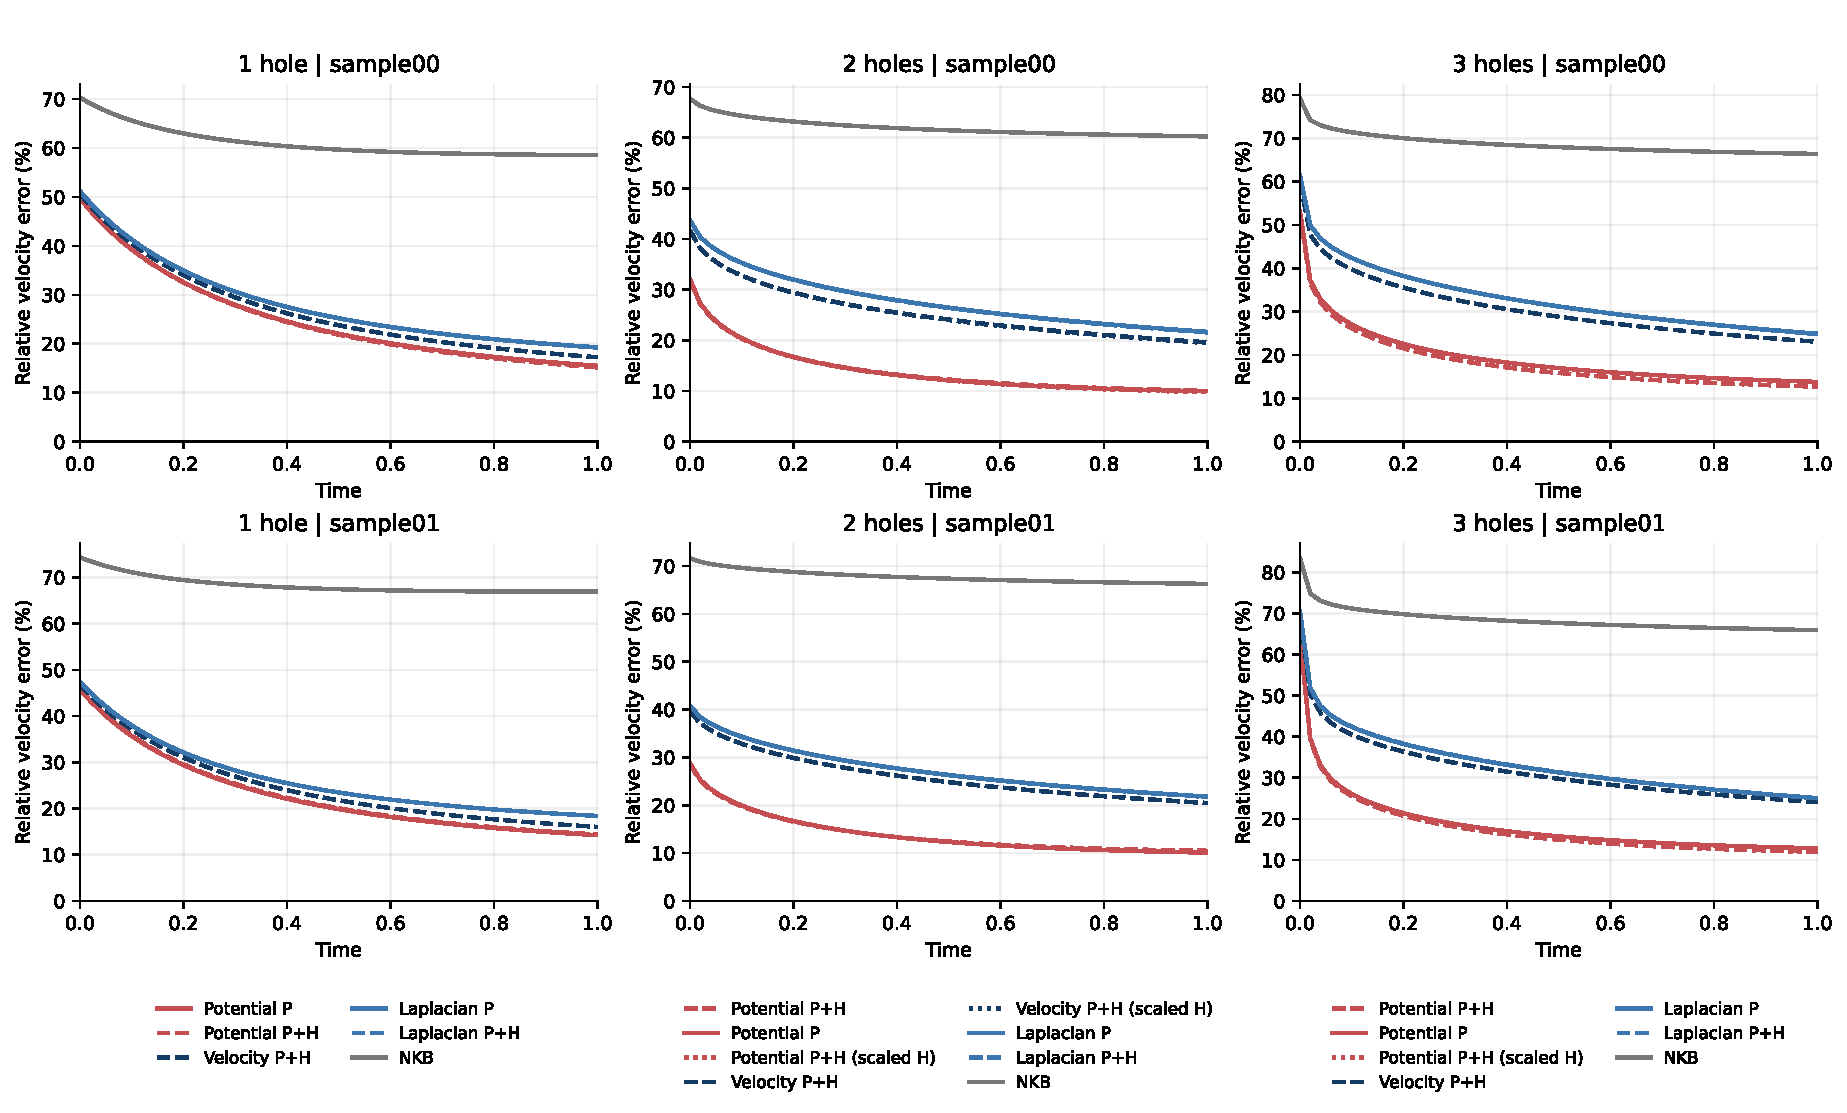
\includegraphics[width=\linewidth,height=.72\textheight,keepaspectratio]{unified_names_20261021_v1/random_k1024_final_velocity_errors.pdf}
\caption{All six autonomous random-field comparisons at $K=1024$ against qualified references. Each panel is one predetermined physical field, and every curve uses all 51 saved times and the original common mask. The numerical control has the same total coordinate count and the corresponding P or P+H allocation.}
\label{fig:random-k1024-errors}
\end{figure}

For a saved coefficient vector, let $M_{\rm assessment}=U^{\top}WU$ denote the full mass matrix on assessment nodes. Its quadratic energy is $c^{\top}M_{\rm assessment}c$ (twice the kinetic energy). Explicit harmonic components are reported both through their own coefficients and as the mass-orthogonal projection of the full velocity onto each method's harmonic span. Let $H$ index the harmonic coordinates, $M_{HH}$ be their mass block, and $\ell_H$ the harmonic entries of the full velocity load. The latter quadratic energy is $\ell_H^{\top}M_{HH}^{-1}\ell_H$, with $\ell_H=(M_{\rm assessment}c)_H$, retaining P/H cross terms. Learned harmonic fields use their original learned representation throughout.

\begin{figure}[htbp]\centering
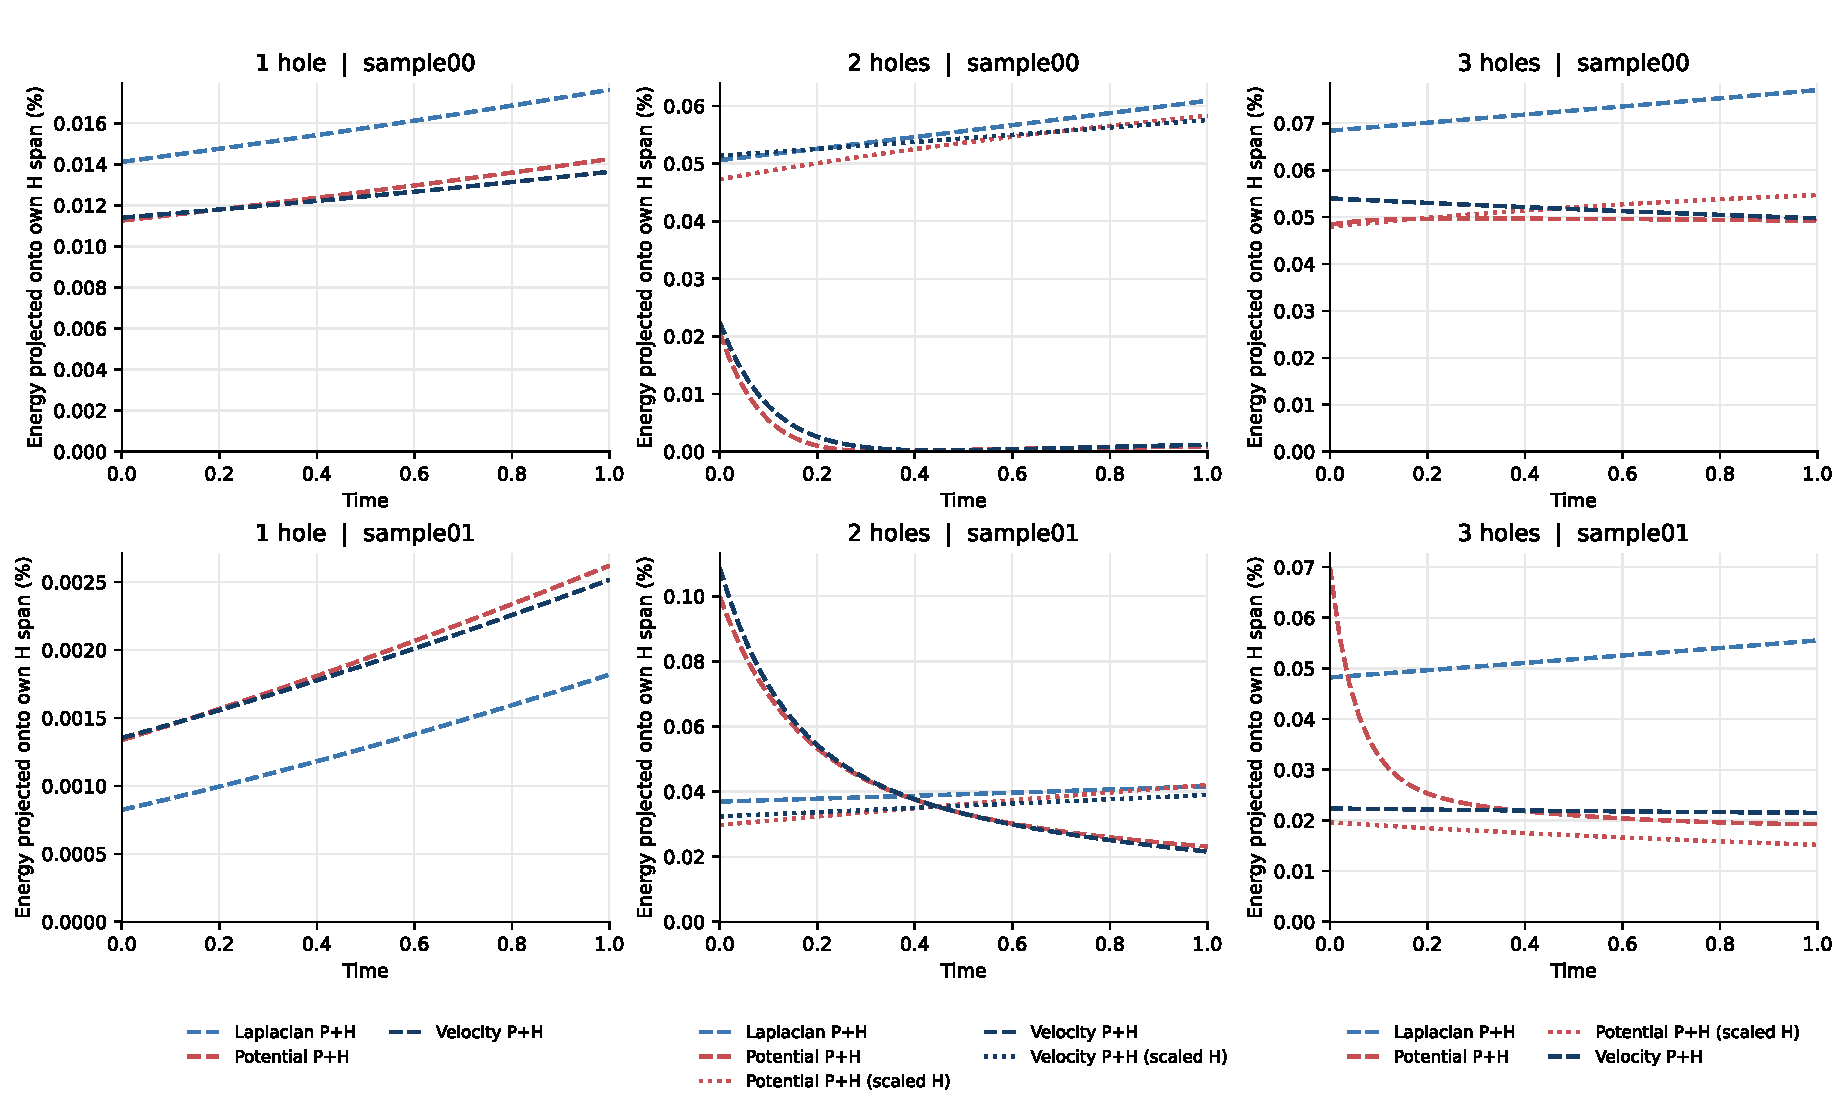
\includegraphics[width=\linewidth,height=.72\textheight,keepaspectratio]{unified_names_20261021_v1/random_k1024_trajectory_harmonic_fraction.pdf}
\caption{Energy projected onto each representation's explicit harmonic span as a fraction of its instantaneous total energy. The projection measures occupation of each representation's explicit circulation coordinates.}
\label{fig:random-k1024-harmonic}
\end{figure}

Supplementary boundary diagnostics use exact edge integration of the original P1 polygon velocities for numerical bases, and nested 1024/2048-point analytic-boundary evaluations for neural bases. They report normal speed and counterclockwise circulation around each enclosed component over all 51 frames. Curl-form neural velocities have cancelling analytic mixed derivatives; NKB divergence is evaluated from its analytic direct-velocity Jacobian at 1024 deterministic original common-mask points. These component diagnostics complement the full-domain error measurements. The released results include all per-component circulation curves, quadrature-refinement differences, and energy histories.

The timing ledger separates reference generation and qualification, cache/operator recovery, projection, batched evolution, and error assessment. Existing 20-field batch costs remain associated with those batches. Stage and process timers retain their respective workload boundaries. Supplementary boundary diagnostics required 390.59 seconds across their measured stages, independently of reference generation and final full-domain error assessment.



\subsection{Three-dimensional dynamics and error attribution}
\label{app:3d-error}
The $128^3$ reference uses rotational NS with viscosity $0.00025$ and normal penalization. The reference solver uses {classical RK4 advection \citep{butcher2008numerical}} with split viscosity and normal-penalty updates at step $0.0025$. Reduced trial fields are zero-extended in the solid and integrated with the projected, unsplit grid generator at $0.00125$ and $0.000625$. Numerical fields use the mapped fitted N\'ed\'elec basis {\citep{nedelec1980mixed}}; learned velocities use analytic curls. All fluid nodes enter the mass matrix, projections, and error measurements. The \hyperref[app:coefficient-acceleration]{coefficient timing study below} additionally evaluates the NS reference at the matched step $0.000625$.

The velocity capacity study retains 6144 training points per epoch, eight validation geometries with 4096 points each every 25 epochs, and all 2000 epochs. Training takes 5361.59 and 8622.13 seconds at $K=128,256$. The learned final/initial energy ratios are $0.496797,0.505110$; numerical ratios are $0.410710,0.396369$. Maximum relative mass-norm time-step differences are below $5.3\times10^{-13}$.

For frozen $U$, let $c_\star(t)$ minimize $\norm{Uc-u_{\rm ref}(t)}$. Projection orthogonality gives
\begin{equation}
\frac{\norm{Uc(t)-u_{\rm ref}}^2}{\norm{u_{\rm ref}}^2}
=\frac{\norm{Uc_\star-u_{\rm ref}}^2}{\norm{u_{\rm ref}}^2}
+\frac{\norm{U(c(t)-c_\star)}^2}{\norm{u_{\rm ref}}^2}.
\label{eq:error-split}
\end{equation}
The representation term decreases with capacity, whereas the in-span term stays close to one half of the reference norm at $K=512,1024$. Its share of the total squared error consequently increases. The decomposition is evaluated after autonomous integration using the saved trajectories and common reference loads. At $K=128,256$, the numerical best-projection errors are $0.659617,0.547576$ and in-span errors are $0.378547,0.414556$, respectively. These controls show the same separation between improving the spatial span and changing its autonomous evolution.

\begin{table}[!htb]\centering\small
\caption{Final orthogonal error decomposition for the velocity-trained Eigenfluid spans, $T=1.16$. Entries are relative velocity errors (\%), normalized by the common full-fluid NS state. Representation and in-span terms add in square, as in \doceqref{eq:error-split}. The $K=512,1024$ entries extend the decomposition using saved full-mass matrices, all 30 reference loads, and autonomous coefficients; their final total errors also agree with direct saved-field differences.}
\label{tab:3d-error-attribution}
\begin{tabular}{rrr}\toprule
$K$ & Best representation & In-span evolution\\\midrule
128 & 67.0459 & 44.5447\\
256 & 55.5999 & 45.6442\\
512 & 43.9777 & 49.7599\\
1024 & 35.0357 & 49.6553\\
\bottomrule\end{tabular}\end{table}


\section{Three-dimensional capacity, computation, and transfer}
\label{app:3d-controls}
\subsection{High-capacity initial representation and training cost}
\label{app:3d-high-capacity}
{The fixed-domain velocity models at $K=512,1024,2048$ each receive 2000 training epochs. Full-mass projection of the common initial numerical velocity on all 1,599,754 fluid nodes gives relative errors of $20.95\%,17.05\%,15.62\%$, compared with $19.65\%,17.90\%,17.27\%$ for the same-capacity Laplacian bases. Doubling learned capacity from 1024 to 2048 reduces initial error by a further 1.43 percentage points and yields an error 1.65 points below the matched numerical control (\docref{Table}{tab:initial2048}). \docref{Figure}{fig:case3-initial-capacity} relates these representation measurements to the training cost.}

\begin{figure}[!htb]
\centering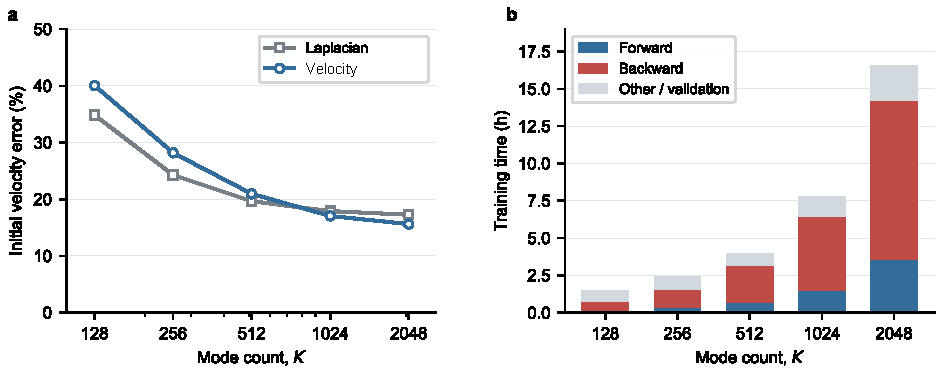
\includegraphics[width=\linewidth,height=.72\textheight,keepaspectratio]{unified_names_20261021_v1/case3_initial_capacity_training.pdf}
\caption{\textbf{Initial representation and training cost in three dimensions.} (a) Full-mass initial projection error on all fluid nodes, using every mode. {Numerical Laplacian and learned velocity results both extend through $K=2048$ and measure initial representation.} (b) Wall time for 2000 epochs: forward and backward computation plus other training costs, including validation and checkpoint I/O. Total times at $K=512,1024,2048$ are 3.99, 7.77, and 16.55 hours.}
\label{fig:case3-initial-capacity}
\end{figure}

\begingroup
\paragraph{Matched $K=2048$ initial representation.}
At 2048 coordinates, the learned velocity basis captures $97.561\%$ of the initial kinetic energy, compared with $97.018\%$ for the same-mesh Laplacian basis (\docref{Table}{tab:initial2048}). Full-mass projections of the common NS initial field retain every mode and all 1,599,754 fluid nodes. The Laplacian modes solve the consistent-mass eigenproblem with relative residuals below $10^{-6}$; the mapped mass agrees with its 1024-mode prefix to $10^{-10}$. Independent direct-field errors and quadratic projection energies agree with $\eta=1-e_0^2$ to $10^{-10}$.
\begin{table}[!htb]\centering\small
\caption{Initial velocity representation at $K=2048$. Learned and Laplacian bases project the same NS initial field with the full mass matrix on all fluid nodes. The table gives captured energy; \docref{Figure}{fig:case3-initial-capacity} plots the corresponding initial velocity errors, and \docref{Figure}{fig:case3-capacity} gives autonomous errors through $K=1024$.}
\label{tab:initial2048}
\begin{tabular}{lr}\toprule
Basis & Captured kinetic energy (\%)\\\midrule
Laplacian & 97.018\\
Velocity & 97.561\\
NKB & 95.314\\
\bottomrule\end{tabular}\end{table}\par\endgroup


\subsection{Coefficient-only acceleration of the 3D Galerkin system}
\label{app:coefficient-acceleration}
For the original $128^3$ normal-penalty generator, let $B_i$ denote a sampled learned velocity field, extended by zero outside the fluid nodes, and let $P_h$ be the original self-adjoint Leray, dealiasing, and zero-mean projector. Here $\Omega_h$ is the set of fluid grid nodes, $h=1/128$ the Cartesian grid spacing, and $\nabla_h,\Delta_h$ the grid spectral gradient and Laplacian. The spatial weight $\chi$ and positive penalty timescale $\eta$ specify the original normal penalty along wall normal $n$. The operators in \doceqref{eq:offline-rom} are
\begin{align}
M_{ij}&=h^3\sum_{x\in\Omega_h}B_i(x)\cdot B_j(x),\\
A_{ij}&=\left\langle B_i,P_h\left[\nu\Delta_h B_j-\frac{\chi}{\eta}(B_j\cdot n)n\right]\right\rangle_h,\\
\mathcal Q_{ijk}&=h^3\sum_{x\in\Omega_h}(P_hB_i)(x)\cdot\left[B_j(x)\times(\nabla_h\times B_k)(x)\right].
\end{align}
The full-grid projector and derivatives act before restriction to the fluid nodes. The adjoint projector in the last line moves the output projection onto the test field, permitting blocked matrix products without changing the nonlinear operator. Input pairs are stored as $j\leq k$, summing $\mathcal Q_{ijk}+\mathcal Q_{ikj}$ for $j<k$. This stores $K^2(K+1)/2$ FP64 entries. All 1,599,754 fluid nodes and all modes are retained; the sampled basis cache remains at its original FP32 precision, with operator construction and coefficient arithmetic in FP64.

At $K=512$, the packed tensor occupies 0.501 GiB and remains on the GPU. Native CuPy evaluation of two production right-hand sides agrees with full-grid projection to $1.17\times10^{-14}$ relative error; one RK4 step differs by $4.53\times10^{-17}$ in relative mass norm. The complete coarse-step trajectory agrees with the full-grid Galerkin trajectory to $1.25\times10^{-14}$. These comparisons verify that tensor assembly preserves the selected reduced dynamics.

On an NVIDIA RTX 4080 SUPER, the 1856 RK4 steps with $\Delta t=0.000625$ to $T=1.16$ take 7.03 seconds. The original numerical NS solver takes 124.75 seconds for the same step size, physical interval, and initial physical field. It retains its split viscosity and normal-penalty integrator; the ROM integrates the projected unsplit generator using RK4. The measured $17.74\times$ ratio compares online integration, including GPU synchronization. Quadratic assembly takes 3645.51 seconds offline; reconstructing and diagnosing three selected frames takes a further 20.41 seconds. Training, derived-field preparation, reference projection, and output are accounted for separately from online integration.

Halving the ROM time step changes the trajectory by at most $2.67\times10^{-12}$ in relative mass norm, confirming temporal convergence of the assembled dynamics. Refining the NS reference from $0.0025$ to $0.000625$ changes its final velocity by $2.12\%$. \docref{Figure}{fig:coefficient-acceleration} presents the flow error and kinetic energy alongside the measured online and preparation costs, characterizing the accuracy--cost tradeoff of coefficient-space execution.
\begin{figure}[!htb]
\centering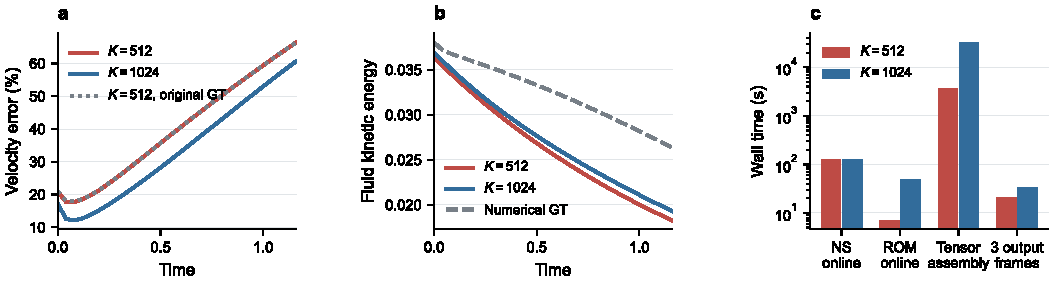
\includegraphics[width=\linewidth,height=.72\textheight,keepaspectratio]{unified_names_20261021_v1/case3_coefficient_acceleration.pdf}
\caption{\textbf{Accuracy, energy, and cost of coefficient-space dynamics.} Red and blue denote $K=512$ and $1024$. (a) Autonomous velocity errors against the shared refined NS reference on all 1,599,754 fluid nodes; the dotted gray curve assesses $K=512$ against the original reference. (b) Fluid kinetic energy. (c) Synchronized NS/ROM online integration, offline tensor assembly, and three-frame output times. Both 2000-epoch models use full-mass initial projection, all retained coordinates, and $\Delta t=0.000625$. Time-step checks are given in the adjacent text; \docref{Table}{tab:coefficient-capacity} reports cost ratios.}
\label{fig:coefficient-acceleration}
\label{fig:coefficient-capacity}
\end{figure}

\paragraph{Capacity scaling of the assembled ROM.}
Increasing velocity-basis capacity improves autonomous accuracy while increasing online integration cost ({\docref{Table}{tab:coefficient-capacity}}). {\docref{Figure}{fig:coefficient-capacity}} shows the corresponding full-fluid error and energy trajectories. All trained coordinates are retained. Packed FP64 tensors occupy 0.501 and 4.004 GiB and remain on the GPU throughout integration. The $K=2048$ measurement in {\docref{Figure}{fig:case3-initial-capacity}} evaluates initial representation.
\begin{table}[!htb]\centering\small
\caption{Coefficient-ROM capacity scaling at $\Delta t=0.000625$, $T=1.16$. \docref{Figure}{fig:coefficient-capacity} shows accuracy against the matched-step NS reference. Assembly measures the offline tensor construction, excluding training and field preparation. Synchronized online NS/ROM wall times define the speed ratio.}
\label{tab:coefficient-capacity}
\begin{tabular}{rrrrr}\toprule
$K$ & Assembly (h) & ROM (s) & NS (s) & Speedup\\\midrule
512 & 1.01 & 7.03 & 124.75 & 17.74$\times$\\
1024 & 9.01 & 48.59 & 126.68 & 2.61$\times$\\
\bottomrule\end{tabular}\end{table}

\paragraph{Operator agreement and stage costs.}
At $K=1024$, assembled and direct full-grid right-hand sides agree to $3.81\times10^{-14}$ relative error; the one-step RK4 discrepancy is $6.48\times10^{-17}$ in relative mass norm. Halving the ROM step changes the trajectory by at most $1.49\times10^{-11}$. {\docref{Appendix}{app:runtime}} collects field preparation, tensor assembly, loading, full-grid checks, projection, and output costs alongside the NKB and Laplacian comparisons. The agreement measurements show that assembly preserves the reduced generator, connecting the online cost directly to the learned span and projected dynamics assessed above.


\subsection{Randomized-field representation across capacities}
\label{app:randomfield-values}
\begin{table}[!htb]\centering\small
\caption{Relative velocity $L^2$ reconstruction errors (\%) on the same 20 independent random large-eddy fields. Entries are mean $\pm$ sample standard deviation, using all 1,599,754 fluid points and all retained modes. These are the numerical values for \docref{Figure}{fig:case3-Pot-capacity}. A dash denotes an unavailable measurement.}
\label{tab:mainfour-NEW20-values}
\begin{tabular}{rcccc}\toprule
$K$&Potential&Velocity&Laplacian&NKB\\\midrule
32&$65.82\pm4.06$&$76.46\pm4.65$&$65.92\pm4.04$&$78.98\pm4.30$\\
64&$49.27\pm4.85$&$60.20\pm4.36$&$49.28\pm4.78$&$73.03\pm3.26$\\
128&$34.39\pm3.95$&$41.96\pm5.36$&$34.59\pm3.85$&$66.67\pm3.81$\\
256&$26.11\pm3.98$&$31.26\pm5.96$&$26.51\pm3.95$&$56.04\pm2.71$\\
512&$23.73\pm3.99$&$26.25\pm5.56$&$23.91\pm4.05$&$41.49\pm2.13$\\
\bottomrule\end{tabular}
\end{table}


\subsection{Differentiable auxiliary gauge projection}
The Potential-FG configuration uses 441 effective scalar gauge directions for differentiable representative selection. A pure-gauge injection diagnostic quantifies the resolved gradient content, with 43.80\% amplitude retained after projection. Scalar corrections preserve the analytic curl exactly. The \hyperref[app:gauge-solvers]{solver comparison below} separately examines refinement, harmonic orthogonality, and derivative consistency using a frozen 32-network auxiliary-solver checkpoint after five updates; it is not the full-training Potential or Potential-FG capacity checkpoint.

\subsection{Potential-AL and Potential-FG controls and capacity}
\label{app:old-Pot}
Potential-AL and Potential-FG are the noncanonical 3D potential controls. The Potential-AL models at $K=32,64,128$ use divergence and wall constraints with an augmented-Lagrangian objective. The seed-0 $K=256$ Potential-FG model uses finite scalar/harmonic gauge projection. Their original-field reconstruction results appear in \docref{Table}{tab:finite-potential-initial}. A separately trained, matched Potential-FG family spans $K=32,64,128,256$, with the results below.

The matched finite-gauge family completes 2000 training epochs and 80 scheduled validations at each of $K=32,64,128,256$. Every model reconstructs the same 20 independent random vortical fields with all retained modes and all 1,599,754 fluid points. At $K=256$, the mean relative $L^2$ errors are 0.910006 for Potential-FG and 0.265110 for the same-capacity Laplacian eigenbasis. The corresponding raw-boundary-to-all-basis times are 291.39, 346.78, 451.21, and 665.15 seconds across the four capacities. These measurements include geometry preparation and streamed basis-output I/O.

\begin{figure}[!htb]
\centering
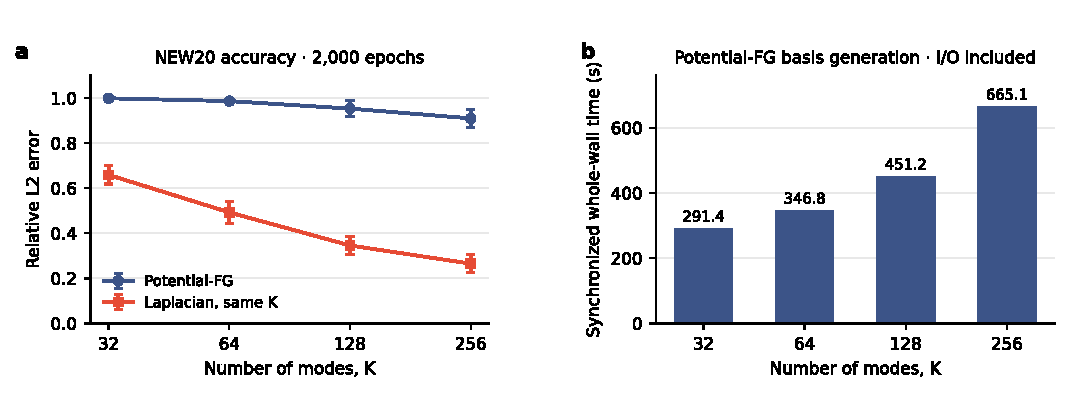
\includegraphics[width=\linewidth]{unified_names_20261021_v1/FG_matched_NEW20_method_names_20261021_v1.pdf}
\caption{\textbf{Matched finite-gauge reconstruction and basis generation.} (a) Relative velocity $L^2$ reconstruction error on 20 independent random vortical fields, using Potential-FG models trained for 2000 epochs and 80 scheduled validations and the same-capacity Laplacian eigenbasis. Error bars show sample standard deviation across the 20 fields. (b) Potential-FG synchronized wall time from raw-boundary JSON parsing and FP64 geometry upload to all 1,599,754 points and all $K$ raw analytic FP64 basis values, including streamed output I/O.}
\label{fig:matched-FG-NEW20}
\end{figure}

\begin{table}[!htb]\centering\small
\caption{Matched Potential-FG reconstruction on the same 20 independent random large-eddy fields, after 2000 epochs and 80 scheduled validations. Relative velocity $L^2$ errors are reported as mean $\pm$ sample standard deviation (\%); all 1,599,754 points and all $K$ modes are retained. The Laplacian entries use the same fields and capacity.}
\label{tab:matched-FG-NEW20-values}
\begin{tabular}{rcc}\toprule
$K$&Matched Potential-FG&Laplacian\\\midrule
32&$99.928\pm0.045$&$65.924\pm4.039$\\
64&$98.690\pm1.315$&$49.278\pm4.782$\\
128&$95.348\pm3.671$&$34.595\pm3.852$\\
256&$91.001\pm4.096$&$26.511\pm3.946$\\
\bottomrule\end{tabular}
\end{table}

\begin{table}[!htb]\centering\small
\caption{Initial relative velocity $L^2$ errors on the original common initial field ($n=1$ per method and capacity), using all retained modes and all 1,599,754 fluid nodes. Potential completes 2000 epochs and 80 scheduled validations through $K=512$. The controls use Potential-AL at $K=32,64,128$ and Potential-FG at $K=256$. The $K=1024$ and $2048$ Potential training runs complete 25 and one optimizer updates, respectively; their completed update counts are reported separately from the full-training representation results.}
\label{tab:finite-potential-initial}
\begin{tabular}{rrrrr}\toprule
$K$&Potential&Velocity&Laplacian&Potential-AL/FG\\\midrule
32&0.843112&0.839273&0.845281&0.917776 (AL)\\
64&0.515772&0.622647&0.521114&0.878704 (AL)\\
128&0.343194&0.400527&0.348509&0.869497 (AL)\\
256&0.235699&0.281845&0.242727&0.994937 (FG)\\
512&0.201610&0.209542&0.196530&\textemdash\\
1024&\textemdash&0.170499&0.178991&\textemdash\\
2048&\textemdash&0.156175&0.172679&\textemdash\\
\bottomrule\end{tabular}\end{table}

The finite projection leaves gradient directions in the curl kernel. For the admissible analytic potential $A=\nabla[e(x)^2\sin(2\pi f(x_1+2x_2+3x_3))]$, where $e$ is the boundary envelope, curl vanishes and $A$ is zero on the boundary. At $f=4$, the scalar and harmonic correction leaves $99.86\%$ of its source-point mass, despite a scalar-system residual below $5\times10^{-15}$. Residual gradient content can enlarge the potential quotient's denominator without adding velocity energy. On the frozen 256-mode model, replacing 441 scalar directions with a nonnested 1392-direction space changes retained potential mass by $44.91\%$ and the mean orthogonalized quotient by a factor of $4.62$, while preserving each raw curl. This measures representative sensitivity rather than auxiliary-space convergence. The measured FP32/FP64 analytic-curl discrepancy is $0.0111\%$. For the Potential-FG seed-0 control, these probes connect finite-gauge sensitivity to its velocity representation; they are not diagnostics of the distinct Potential-AL loss. Full-mass best projection is invariant to nonzero column scaling, so reduced curl amplitude alone does not explain the reconstruction error. Resolving gradient content is the necessary qualification for this 3D potential objective.

\subsection{Accuracy and cost of the auxiliary gauge solve}
\label{app:gauge-solvers}

The auxiliary solve selects the potential representative entering the Rayleigh quotient. Its accuracy depends on the space used to represent the Poisson correction as well as on the precision of the linear algebra. We compare these effects on a fixed 32-network checkpoint obtained after five updates with Fourier projection and a method-of-fundamental-solutions (MFS) boundary correction. All methods use the same smooth Metaball geometry, neural parameters, analytic derivatives, and relative harmonic field, isolating representative selection from learning.

\paragraph{Common assessment.}
Let $A_\theta$ denote the neural vector potential, with raw column $A_j$. Its scalar divergence forcing is $f_j=\diver A_j$, and $\phi_j$ denotes its numerical scalar correction. We define $\epsilon_P$ as the maximum relative Poisson residual over columns $j=1,\ldots,32$; the sums below use unit weights on independent points $x_q$. On 8192 identical independent fluid points, we report
\begin{equation}
\epsilon_P=\max_{j\leq32}
\frac{\left(\sum_q|f_j(x_q)-\Delta\phi_j(x_q)|^2\right)^{1/2}}
{\left(\sum_q|f_j(x_q)|^2\right)^{1/2}}.
\label{eq:gauge-solver-residual}
\end{equation}
The residual measures the fraction of divergence forcing left after the scalar correction, since $\diver(A_j-\nabla\phi_j)=f_j-\Delta\phi_j$. Relative harmonic overlap is measured on a disjoint 110592-node volume rule after the column transform, and tangential trace on 8192 independent points per wall. Columnwise diagnostics characterize gradient correction, harmonic orthogonality, and boundary trace across all 32 modes. Setup, forward, reverse, and assessment times are measured separately on an RTX 4080 SUPER using native CuPy. Forward/reverse measurements use a 4 GiB allocation pool; the R-marked synchronized setup and assessment measurements use a 12 GiB pool with the same complete workload.

\paragraph{Fourier particular solution and boundary correction.}
On an auxiliary box of side $L=1.12$, an exterior continuation agrees with the original neural potential throughout the fluid. Its divergence is sampled on $193^3$ nodes. Let $k\in\mathbb Z^3$ be an integer wavevector ($\mathbb Z$ denotes integers), $\kappa_k=2\pi k/L$ its physical frequency, $x_0$ the box origin, and $\widehat f_k$ the Fourier coefficients of the sampled forcing. The scalar particular solution $\phi_p$ is
\begin{equation}
\phi_p(x)=-\sum_{k\ne0}\frac{\widehat f_k}{|\kappa_k|^2}
e^{\mathrm i\kappa_k\cdot(x-x_0)}
+\widehat f_0\frac{|x-(0.5,0.5,0.5)|^2}{6}.
\end{equation}
The mean term preserves nonzero-mean forcing. The represented Laplacian is the Fourier interpolant $f_N$ with $N=193$ nodes per axis. The independent residual $f_j-f_N$ measures the source representation at this resolution. A Laplace method-of-fundamental-solutions (MFS) correction with 6144 exterior sources and 18432 boundary collocation nodes enforces the zero Dirichlet trace in least squares \citep{fairweather1998method}. This harmonic boundary correction complements the volume particular solution. We separately test the training arithmetic, FP64 fast Fourier transforms (FFTs) on the same FP32 samples, and an FP64 source/FFT path. A reuse control combines repeated source FFTs and accumulates spectral cotangents before the source-grid inverse FFT, keeping the represented operator unchanged.

\paragraph{Smooth weak projection.}
For a scalar test function $v\in H_0^1(\Omega)$, integration by parts gives the same continuous Dirichlet problem in the form
\begin{equation}
\int_\Omega\nabla v\cdot\nabla\phi\,\dd x
=\int_\Omega\nabla v\cdot A_\theta\,\dd x,
\qquad v\in H_0^1(\Omega).
\end{equation}
We use $C^2$ tensor cubic B-splines {\citep{deboor1978splines}} multiplied by the original analytic zero-trace envelope. Let $b_i$ be the enveloped spline basis functions, $\zeta_i$ their coefficients in $\phi_h=\sum_i\zeta_i b_i$, $\zeta=(\zeta_i)$ their coefficient vector, $\mathsf K$ the gradient stiffness matrix, and $r=(r_i)$ the load vector. The discretization is
\begin{equation}
\mathsf K_{ij}=\sum_qw_q\nabla b_i(x_q)\cdot\nabla b_j(x_q),\quad
r_i=\sum_qw_q\nabla b_i(x_q)\cdot A_\theta(x_q),\quad \mathsf K\zeta=r.
\end{equation}
The neural right-hand side and its parameter reverse require potential values rather than divergence derivatives. Basis gradients and Laplacians are analytic, including across spline knots. Resolution-12, -20, and -24 spaces use 32768, 110592, and 262144 fitting quadrature points. {Matrix-free conjugate gradients \citep{hestenes1952methods} apply the weighted gradient Gram operator; a standard two-level construction \citep{briggs2000multigrid} uses cubic refinement prolongation, symmetric smoothing, and a factored coarse solve.} Severely cut supports are removed when their quadrature gradient-energy diagonal is at most $10^{-5}$ of the maximum. The selection and quadrature remain fixed during differentiation. The algebraic solve residual measures convergence within this space, while \doceqref{eq:gauge-solver-residual} measures the resolved neural forcing.

\paragraph{Volume potential with multipole acceleration.}
{The alternative particular solution follows volume-potential methods \citep{malhotra2016volume} and uses the Newton potential of the piecewise-constant source density $f_h$ over the auxiliary box $B$, with $y$ the integration point:}
\begin{equation}
\phi_p(x)=-\frac1{4\pi}\int_B\frac{f_h(y)}{|x-y|}\,\dd y.
\end{equation}
The volume representation uses constant cuboid densities in $B=[-0.02,1.02]^3$, with the same interior forcing and exterior continuation. Near cuboids, including self interactions, are integrated analytically. {Degree-six Cartesian multipole-to-multipole, multipole-to-local, and local-to-local translations follow the fast multipole method (FMM) \citep{greengard1987fast} to evaluate the far field, whose local Taylor polynomials are harmonic.} The same MFS correction enforces the boundary trace. A source-adaptation variant refines coarse cells when a neighboring density difference, normalized by the per-column coarse-source root mean square (RMS) and maximized over the 32 columns, exceeds $0.5$. The sampling map is fixed for the adjoint, and evaluation uses a uniform tree. The fixed sampling map permits consistent differentiation through the adaptive piecewise-constant representation, following the volume-potential construction \citep{malhotra2016volume}.

% Frozen all-32 checkpoint measurements.
\begin{table}[!htb]\centering\footnotesize\setlength{\tabcolsep}{3pt}
\caption{Gauge-solver accuracy and cost at the fixed checkpoint. \docref{Figure}{fig:gauge-solver-ablation} plots the Poisson residual $\epsilon_P$. Harmonic overlap and tangential trace are percentages; all four timing columns are seconds. Size denotes grid size or retained spline degrees of freedom. Setup and assessment are excluded from forward/reverse. Superscript R denotes a synchronized measurement of the complete workload; forward/reverse columns exclude setup and assessment.}
\label{tab:gauge-solver-ablation}

\begin{tabular}{lrrrrrrr}\toprule
Method&Size&Harm.&Wall tan.&Forward&Reverse&Setup&Assess.\\\midrule
Fourier--MFS & $193^3$ & 0.0177 & 0.6904 & 49.07 & 138.60 & $54.57^{\mathrm R}$ & $23.82^{\mathrm R}$\\
Fourier--MFS, reuse & $193^3$ & 0.0177 & 0.6904 & 48.28 & 136.12 & $62.86^{\mathrm R}$ & $23.32^{\mathrm R}$\\
Spline 12 & 3,106 & 0.0181 & 0.0012 & 6.63 & 6.98 & 1.98 & 5.90\\
Spline 20 & 10,648 & 0.0015 & 0.0012 & 15.40 & 16.60 & 4.75 & 5.91\\
Spline 24 + two-level & 17,086 & 0.0036 & 0.0012 & 71.00 & 78.96 & 11.69 & 5.84\\
Volume FMM 32 & $32^3$ & 0.0242 & 4.8727 & 12.15 & 13.43 & 22.99 & 61.76\\
Volume FMM 64 & $64^3$ & 0.0261 & 3.6399 & 14.23 & 17.66 & 22.82 & 60.63\\
Volume FMM 64 adaptive & $64^3$ & 0.0261 & 3.6399 & 14.53 & 17.96 & 23.71 & 60.51\\\bottomrule\end{tabular}\end{table}

Forward and reverse totals include synchronized component measurements; one-time setup and independent assessment are separate columns. Setup combines spline space/quadrature and optional multigrid construction, or the FMM and fixed harmonic moments; assessment combines independent residual, harmonic, and wall checks. Spline forward timing includes query-point construction. The Fourier and Fourier-reuse measurements share identical neural passes and include source-array export, while spline and volume methods use in-memory sources. Both particular-solution families reuse the geometry-dependent MFS factors.

\begin{table}[!htb]
\centering\small
\caption{Floating-point precision on the same $193^3$ grid. The first two rows use identical source samples. Source time measures one all-32 forward pass, including export.}
\label{tab:gauge-precision}
\begin{tabular}{lrr}\toprule
Arithmetic & $\epsilon_P$ (\%) & Source forward (s)\\\midrule
Training arithmetic & 7.989593 & 37.24 \\
FP32 source, FP64 FFT & 7.989595 & 37.24 \\
FP64 source and FFT & 7.989582 & 266.41 \\
\bottomrule\end{tabular}\end{table}
\paragraph{Representation and arithmetic.}
The precision controls yield nearly identical forcing residuals (\docref{Table}{tab:gauge-precision}). With identical source samples, changing FFT precision produces a relative Laplacian difference of $4.20\times10^{-7}$. Source-space resolution therefore provides the effective control over representative selection at this checkpoint.

Transform reuse preserves forward outputs to the reported precision and changes the source cotangent by a relative $2.50\times10^{-12}$. It reduces the three-evaluation Fourier stage from 9.91 to 8.99 seconds and the source-grid transpose from 12.96 to 10.48 seconds. Total component time decreases from 187.67 to 184.40 seconds (1.74\%); neural source evaluation and parameter differentiation account for 85.5\% of the original total.

\paragraph{Auxiliary-space resolution.}
Refinement systematically improves the spline and volume corrections (\docref{Figure}{fig:gauge-solver-ablation}), while the harmonic projection maintains small overlap across the solver family (\docref{Table}{tab:gauge-solver-ablation}). These complementary diagnostics identify two controls for representative selection: the approximation space resolves gradient content, and the mass projection selects harmonic coordinates. Source adaptation refines 31,432 of 32,768 coarse cells (95.9\%), with 284,224 source evaluations including the coarse pass, compared with 262,144 for the uniform rule. This distribution favors uniform refinement for the present forcing.
\paragraph{Operator consistency.}
FMM evaluation and transpose consistency are tested using $16^3$ cuboids, 48 query points, and two random right-hand sides. The analytic cuboid kernel agrees with nonsingular Gauss integration to relative $7.30\times10^{-11}$. Against direct cuboid integration, increasing the far expansion degree from four to six reduces relative gradient error from $1.38\times10^{-3}$ to $1.90\times10^{-4}$; the degree-six transpose discrepancy is $2.73\times10^{-16}$. These comparisons isolate evaluation of the chosen density from density approximation. For the manufactured scalar $e(x)[1+0.2\sin(2\pi x_1)+0.1x_2x_3]$, the refined spline method gives relative gradient and Poisson errors of $2.85\times10^{-4}$ and $8.82\times10^{-4}$, with linear residual $4.95\times10^{-9}$. Together with \docref{Figure}{fig:gauge-solver-ablation} and \docref{Table}{tab:gauge-solver-ablation}, these checks connect accurate operator evaluation to systematic control through auxiliary-space refinement.

\begin{figure}[!htb]
\centering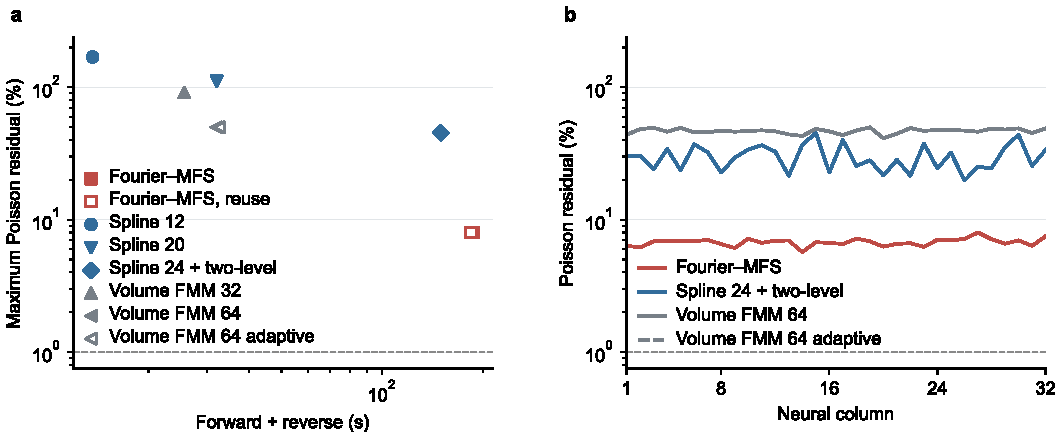
\includegraphics[width=\linewidth,height=.72\textheight,keepaspectratio]{gauge_solver_ablation.pdf}
\caption{\textbf{Gauge-solver accuracy and cost.} Left: all-32 forward-plus-reverse time versus independent Poisson residual. Right: per-column residuals for Fourier--MFS and the finest tested spline and volume spaces. All methods evaluate the same fixed neural checkpoint.}
\label{fig:gauge-solver-ablation}
\end{figure}


\paragraph{Connection to the velocity span.}
At a fixed network, each scalar correction has zero curl, so all solvers retain the same 32-dimensional analytic velocity span. The solver comparison therefore measures representative selection for the potential objective; changes to the learned velocity span arise through subsequent optimization.


\subsection{Training and boundary-to-basis costs}
\label{app:Pot-cost}
\begin{table}[!htb]\centering\scriptsize
\caption{Three-dimensional training and basis-generation costs in seconds. Normal training includes the scheduled validation and checkpoint I/O of each run; state recovery is separate. The reported full training runs complete 2000 epochs. Basis generation measures one synchronized interval from the original parameterized boundary to all 1,599,754 points and all $K$ basis fields, including required streamed-output I/O. The Laplacian interval also includes interstage waits, setup, paging, and background load. Runtime/model loading, coefficient synthesis, projection, and diagnostics have separate boundaries. A dash denotes an unavailable measurement under the stated run and timing boundary; Laplacian has no training or recovery stage. Completed short high-capacity Potential runs are reported in \docref{Table}{tab:CCQ-highK-runtime}. $\dagger$ denotes an inclusive training-time counter. Matched Potential-FG rows complete 2000 epochs and 80 validations; their reconstruction and basis-generation results also appear in \docref{Figure}{fig:matched-FG-NEW20}.}
\begin{tabular}{rlrrr}\toprule
$K$&Method&Normal training&State recovery&Boundary to all basis\\\midrule
32&Laplacian&\textemdash&\textemdash&3467.56\\
32&Velocity&3042.38&0.00&267.91\\
32&Potential&8170.08&200.31&255.50\\
32&Potential-AL&6316.24&0.00&259.52\\
32&Potential-FG (matched)&7332.09&0.00&291.39\\
64&Laplacian&\textemdash&\textemdash&2545.51\\
64&Velocity&3930.13&\textemdash&307.32\\
64&Potential&14404.07&0.00&269.28\\
64&Potential-AL&10513.53&\textemdash&273.65\\
64&Potential-FG (matched)&11924.79&0.00&346.78\\
128&Laplacian&\textemdash&\textemdash&3576.89\\
128&Velocity&5361.59&\textemdash&295.34\\
128&Potential&26569.77&0.00&281.03\\
128&Potential-AL&18887.93&4036.51&281.98\\
128&Potential-FG (matched)&20862.81&0.00&451.21\\
256&Laplacian&\textemdash&\textemdash&\textemdash\\
256&Velocity&8622.13&\textemdash&310.61\\
256&Potential&59879.95&717.31&291.56\\
256&Potential-FG (seed 0)&$23238.19^{\dagger}$&\textemdash&469.61\\
256&Potential-FG (matched)&39108.35&0.00&665.15\\
512&Laplacian&\textemdash&\textemdash&\textemdash\\
512&Velocity&14366.09&\textemdash&488.29\\
512&Potential&504713.77&106.03&348.12\\
512&Potential-AL/FG&\textemdash&\textemdash&\textemdash\\
1024&Laplacian&\textemdash&\textemdash&22049.01\\
1024&Velocity&27976.58&\textemdash&747.68\\
1024&Potential&\textemdash&\textemdash&\textemdash\\
1024&Potential-AL/FG&\textemdash&\textemdash&\textemdash\\
2048&Laplacian&\textemdash&\textemdash&\textemdash\\
2048&Velocity&59575.55&\textemdash&1379.85\\
2048&Potential&\textemdash&\textemdash&\textemdash\\
2048&Potential-AL/FG&\textemdash&\textemdash&\textemdash\\
\bottomrule\end{tabular}
\label{tab:Pot-training-basis-cost}
\end{table}
Initial-field evaluation is separate from training and basis generation: Potential takes 655.76 seconds at $K=256$ and 1182.42 seconds at $K=512$. At $K=512$, the saved-basis assessment of 20 independent random fields takes 123.32 seconds. High-capacity Potential training completes 25 updates at $K=1024$ and one update at $K=2048$, with zero scheduled validations, the original 2000-epoch learning-rate horizon, and full model/Adam endpoint checkpoints.

At $K=1024$, Laplacian construction from raw geometry (marching-cubes resolution 80, mesh size $0.025$) through the full spectrum and coefficient archive takes 18769.83 seconds. The sampled-basis stage takes 477.10 seconds and writes all $1{,}599{,}754\times3\times1024$ FP64 values (39,315,554,304 payload bytes). The raw-geometry-to-output interval is 22049.01 seconds, including interstage waits, setup, paging, I/O, and background load. CPU construction uses one BLAS thread, a 7 GiB resident limit, and an 8 GiB resident-peak guard; GPU basis output reuses the completed analytic geometry prefix.

\begin{table}[!htb]\centering\small
\caption{High-capacity Potential training runtime. Elapsed time runs from the first native training-worker start to atomic publication of the complete model and Adam endpoint. It includes the intervening implementation repairs, recovery, waits, failed attempts and output I/O. Both runs use zero scheduled validations and retain the original 2000-epoch learning-rate horizon.}
\label{tab:CCQ-highK-runtime}
\begin{tabular}{rrr}\toprule
$K$ & Completed optimizer updates & Elapsed runtime (s)\\\midrule
1024&25&13267.46\\
2048&1&69257.03\\
\bottomrule\end{tabular}
\end{table}


\subsection{Training geometry and frequency}
The full 2000-epoch Potential and three-dimensional velocity runs use the original sampling and optimization computations: 6144 query points and eight 4096-point validation geometries every 25 epochs (80 scheduled validations). The high-capacity Potential training runs at $K=1024,2048$ retain the original sampling and learning-rate horizon and complete 25 and one updates with zero scheduled validations. Potential retains the established canonical objective and two-pass causal Gram--Schmidt; its canonical physical actions use FP64, while ANN parameters and analytic derivatives use FP32. The three-dimensional velocity capacity family uses a fixed training domain, first-layer frequency 40, and cosine learning-rate endpoints scaled by 0.1 relative to the original velocity configuration. Its reported checkpoints complete 2000 epochs with the original sampling and scheduled validation. The Potential-AL models at $K=32,64,128$ use seed 20260823, frequencies 40/36, and cosine learning-rate endpoints $2.8\times10^{-5}$ and $10^{-7}$. The Potential-FG $K=256$ model instead uses seed 0, frequencies 160/36, and endpoints $2.8\times10^{-4}$ and $10^{-6}$; it is not a matched cross-method control. \hyperref[app:unseen-geometry]{Geometry-conditioned evaluation on other domains} is reported separately below.


\subsection{Capacity and unseen-geometry reconstruction}
\label{app:unseen-geometry}
\begin{table}[!htb]
\centering\small
\caption{Held-out velocity reconstruction on disjoint 16,384-point assessment sets. Fixed-domain learned checkpoints complete 2000 epochs. Numerical bases use the same capacity, fit and assessment point sets, and target fields. Geometries 2 and 3 use radial Piola transport; geometry 4 uses a globally qualified quadratic approximation of its original smooth boundary and consistent physical finite-element matrices.}
\begin{tabular}{rlrr}\toprule
$K$ & Geometry & Learned & Numerical\\\midrule
128 &Training geometry, independent points&.398468&.346917\\
256 &Training geometry, independent points&.281388&.241861\\
256 &Unseen geometry 2&.751690&.222570\\
256 &Unseen geometry 3&.744673&.254720\\
256 &Unseen geometry 4&.770144&.230048\\\bottomrule
\end{tabular}
\end{table}
The geometry-2 numerical basis uses a fitted mesh with 80,890 vertices and 354,108 tetrahedra, the relative-potential finite-element method (FEM) with consistent mass, and radial Piola transport onto the smooth target domain. Geometry 3 uses the same construction on its own fitted mesh. Each reconstruction uses all 256 positive modes and the identical 16,384 fit points, disjoint assessment points, and target velocities. Solution and reconstruction take 687.17 and 1061.51 seconds for geometries 2 and 3, after mesh and point-map preparation. Geometry 4 retains all 320,815 tetrahedra and uses a quadratic physical N\'ed\'elec chart: positive cell determinants, the entire 95,296-face boundary homotopy, and the boundary degree qualify its global map. This chart approximates the original smooth geometry. Its consistent stiffness/mass eigensolve obtains 264 Ritz vectors with maximum relative residual $5.04\times10^{-11}$; the reconstruction retains 256 positive modes. Assembly, solve, and evaluation total 1054.85 seconds. The disjoint error is .230048, while the fit-point error is .227943. All three learned transfer measurements use the unchanged frozen checkpoint.


\section{Additional paired flow visualizations}
\label{app:fields}
\subsection{Random large-vortex ablations and matched flow views}
These figures report the random large-vortex ensemble used for the $K=1024$ lift-conditioning comparisons in \docref{Section}{sec:case2}. The direct random-streamfunction ensemble is reported separately in \docref{Appendix}{app:random-streamfunction}.
\begin{figure}[!htb]
\centering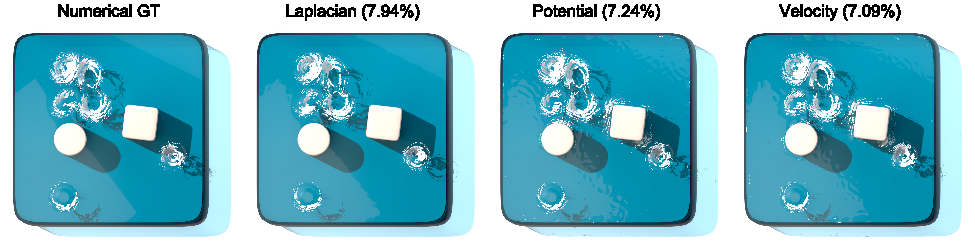
\includegraphics[width=\linewidth,height=.72\textheight,keepaspectratio]{unified_names_20261021_v1/case2_h2_k1024_fourway_houdini.pdf}
\caption{\textbf{Random large-vortex flow around two holes with a shared harmonic lift.} Numerical reference, Laplacian, potential-trained, and velocity-trained trajectories at $K=1024$, $t=1$, seed 1, state 00. Both learned bases use scaled $H_2$. Shared height and contour mappings preserve amplitude differences; annotations give full-domain velocity error.}
\label{fig:case2-velocity-water}
\end{figure}

\begin{figure}[!htb]
\centering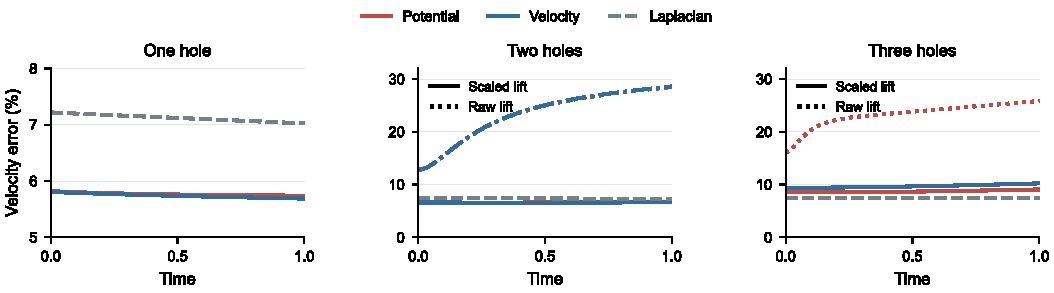
\includegraphics[width=\linewidth,height=.72\textheight,keepaspectratio]{unified_names_20261021_v1/case2_ablations.pdf}
\caption{\textbf{Harmonic completion, lift conditioning, and objective choice.} One-, two-, and three-hole trajectories use total-$1024$ bases and average the same 20 random large-vortex states. Red/blue denote potential/velocity learning, dashed gray numerical completion, dotted red raw lifts, and dash-dot blue the raw-$H_2$ velocity control. Matched learned bases share raw $H_1$, scaled $H_2$, and scaled $H_3$. Curve endpoints give the final-error comparison; positive-basis training costs appear in \docref{Table}{tab:runtime-training}.}
\label{fig:case2-ablation}
\end{figure}


\subsection{Periodic matched-basis comparison}



\paragraph{Periodic vortex-merger relief.}
\docref{Figure}{fig:case1-field} uses saved potential-trained $K=1024$, seed-0 states at $t=0,9\pi,18\pi$ from the $d=1.35$ trajectory. On the periodic $384^2$ display grid, $S$ smooths $|\omega|$ with Gaussian standard deviation 4.5 pixels; all three times use the fixed original scale $q=0.7395528286634208$ and the common display height $h=0.20-1.40[\operatorname{clip}(S|\omega|/q,0,1)]^{0.70}$. Here $\operatorname{clip}(v,a,b)$ clamps $v$ to $[a,b]$. One subdivision smooths the display mesh. At the middle time, white foam follows 12 signed-smoothed vorticity contour levels, normalized by the same fixed $q$, from 0.065 to 0.69; this exposes the elongated S-shaped merger filaments and pointed outer lobes. At the initial and final times, continuous spiral material accents are anchored to measured vortex cores and cover both deep and shallow relief. These material cues emphasize vortex structure on the data-derived height surface. The oblique camera, lighting, transparent water material, and white ground are shared. Saved velocity, vorticity, and ROM coefficients are unchanged.

\begin{figure}[!htb]
\centering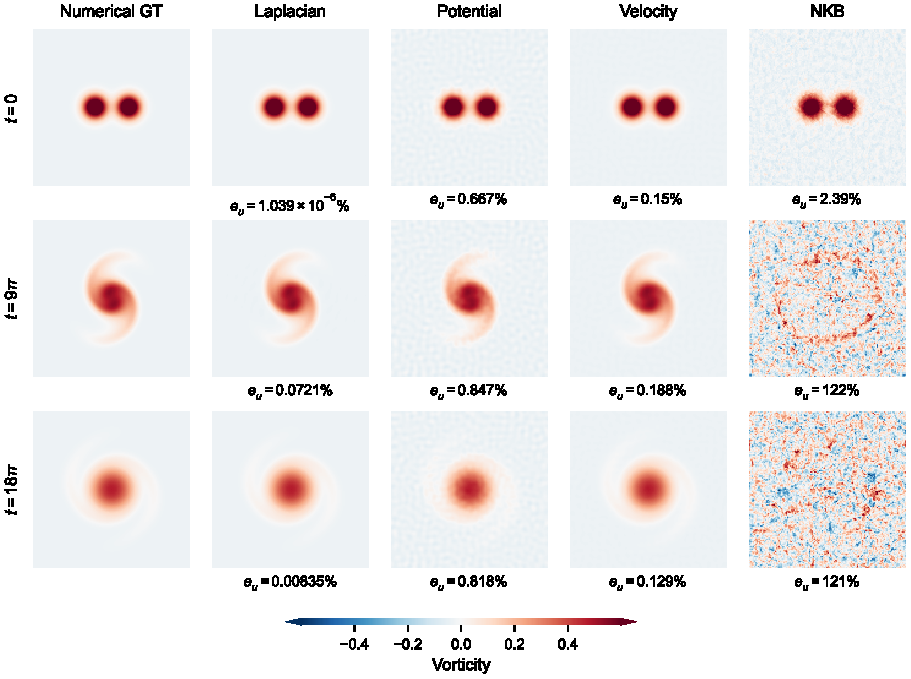
\includegraphics[width=\linewidth,height=.72\textheight,keepaspectratio]{unified_names_20261021_v1/case1_matched_fields.pdf}
\caption{\textbf{Vortex merger at $K=1024$.} Columns compare Numerical GT, Laplacian, potential-trained, velocity-trained, and NKB bases; rows show $t=0,9\pi,18\pi$. Learned fields use seed 0 and maximum step $0.005$. Signed vorticity uses the common GT 99.5th-percentile scale; colorbar extensions indicate saturation. Annotations report velocity error over the full $128^2$ observation grid. All methods use the same $d=1.35$ initial velocity and evolve autonomously.}
\label{fig:case1-fourway}
\end{figure}

\subsection{Three-dimensional flow comparison}
\docref{Figure}{fig:3d-context} compares instantaneous velocity streamtubes for the numerical reference, Laplacian basis, and velocity-trained Eigenfluid basis. Shared camera, seeding, material, and speed mapping expose the three-dimensional flow structure behind the common-slice comparison in \docref{Figure}{fig:case3-field}.
\begin{figure}[!htb]
\centering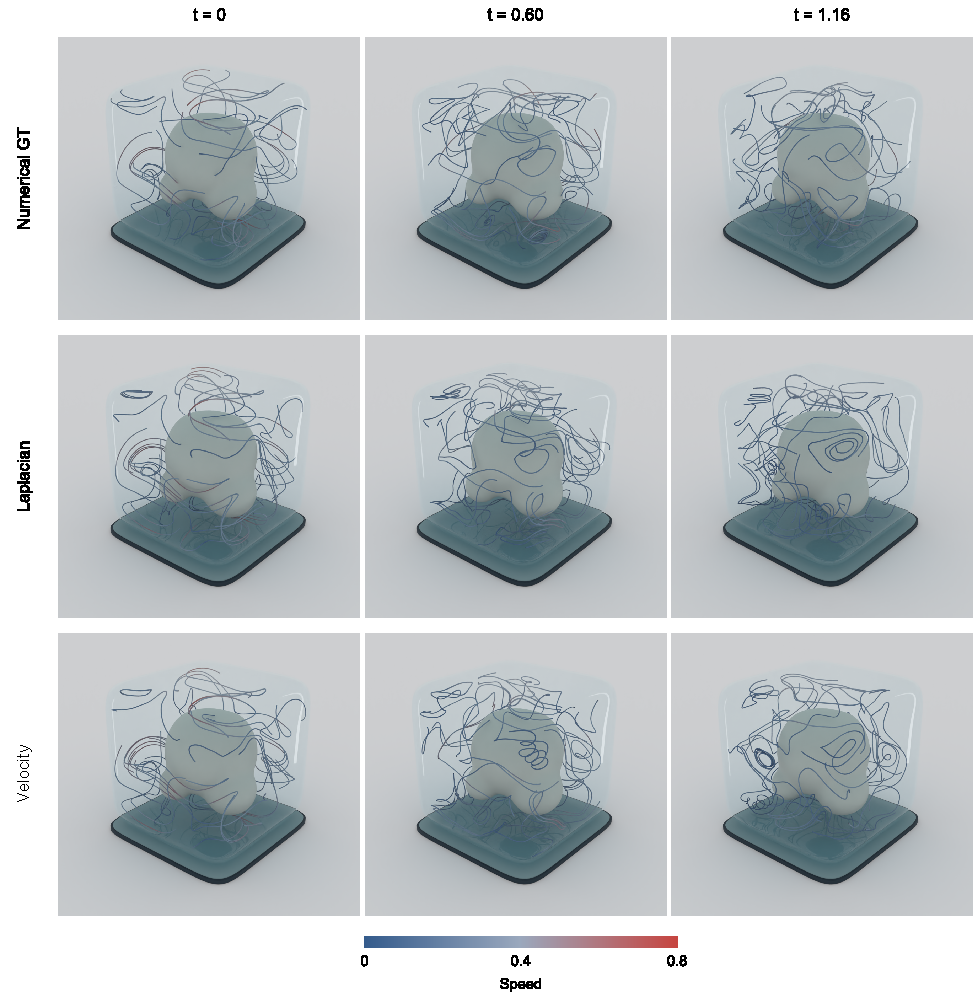
\includegraphics[width=\linewidth,height=.72\textheight,keepaspectratio]{unified_names_20261021_v1/case3_houdini_glass_3d.pdf}
\caption{\textbf{Three-dimensional flow structure.} Numerical GT, Laplacian, and velocity-trained Eigenfluid $K=1024$ streamtubes at $t=0,0.60,1.16$, colored by speed. The transparent shell follows the rounded domain boundary. Camera, seeding, material, and the $[0,0.8]$ speed range are shared. Centerline smoothing is a display operation.}
\label{fig:3d-context}
\end{figure}

\subsection[Three-hole K1024 time sequence]{Three-hole $K=1024$ time sequence}
\docref{Figure}{fig:case2-h3-water-time} follows the refined reference and all three completed bases through three saved times. One display mapping across methods and times preserves temporal changes in the surface relief.
\begin{figure}[!htb]
\centering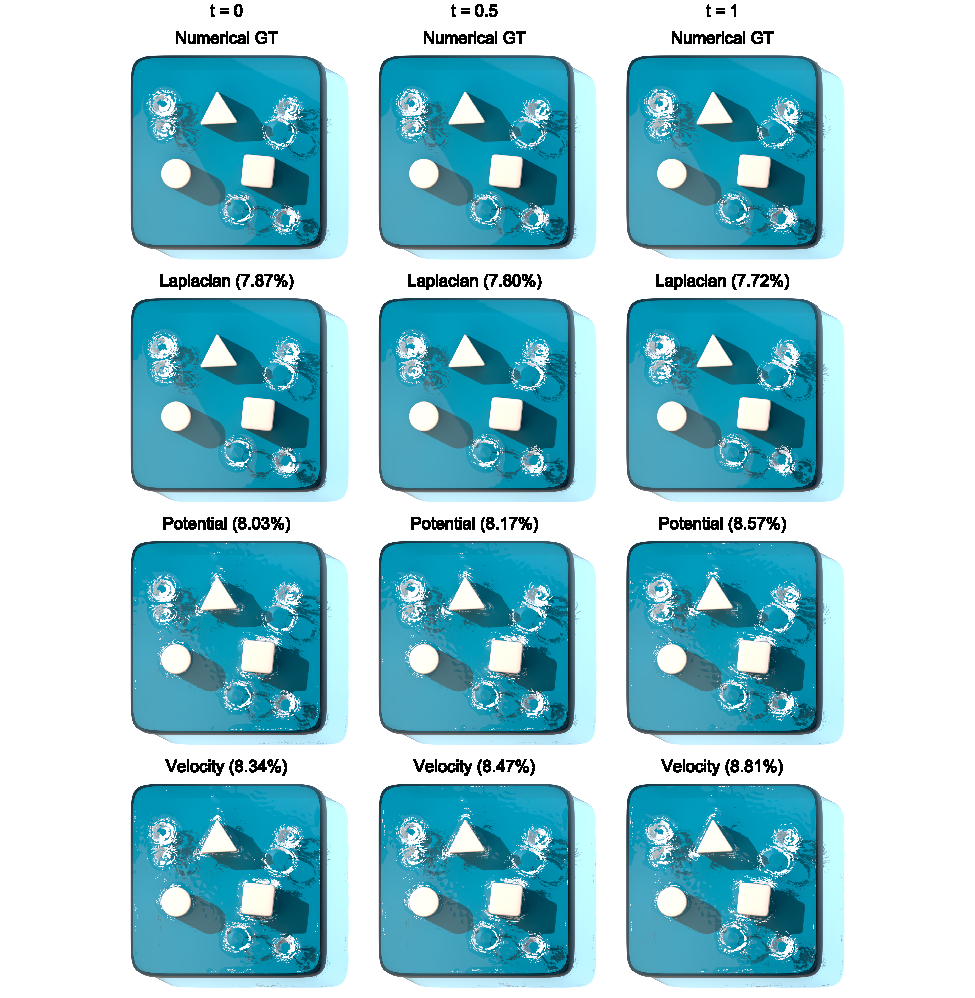
\includegraphics[width=\linewidth,height=.72\textheight,keepaspectratio]{unified_names_20261021_v1/case2_h3_k1024_fourway_houdini_sequence.pdf}
\caption{\textbf{Three-hole evolution at $K=1024$.} Rows compare Numerical GT, Laplacian, potential-trained, and velocity-trained bases; columns show $t=0,0.5,1$, seed 1, state 00. Each basis contains 1021 positive and three harmonic coordinates; the learned bases share scaled $H_3$. All panels share the height mapping, contour levels, camera, and material. Annotations give full-domain velocity error against the level-2 reference.}
\label{fig:case2-h3-water-time}
\end{figure}


\paragraph{Water-surface display mapping.}
The $K=1024$ renderings in \docref{Figures}{fig:case2-field}, \ref{fig:case2-velocity-water}, and~\ref{fig:case2-h3-water-time} embed the saved two-dimensional fields in a height surface. Analytic derivatives of the learned fields are evaluated from the original checkpoints and contracted with the saved coefficients. The refined GT vorticity is recovered from its stored streamfunction using the original interior finite-element mass--stiffness relation. On a $481\times481$ display grid, let $S$ be a masked Gaussian smoother with standard deviation 8 pixels. Let $Q_p[f]$ be the pooled empirical quantile of field $f$ at probability $p$, $q$ a combined vorticity--speed display signal, and $z_{\rm disp}$ the display height. Define
\begin{align*}
q&=0.8\,\frac{|S(\omega)|}{Q_{0.90}[|S(\omega)|]}
  +0.2\,\frac{S(\|u\|^2)}{Q_{0.90}[S(\|u\|^2)]},\\
z_{\mathrm{disp}}&=0.30-0.75\,\operatorname{clip}\!\left(
\frac{q-Q_{0.02}[q]}{Q_{0.98}[q]-Q_{0.02}[q]},0,1\right).
\end{align*}
Quantiles pool all four methods and all three times within each geometry; the main views and time sequence reuse that common mapping. Filtering signed vorticity before taking its magnitude emphasizes coherent large-scale structure. The speed term also reveals curl-free harmonic circulation. Height is a display coordinate; the saved physical fields and ROM coordinates remain unchanged. White foam follows shared streamfunction contour levels after subtracting each field's nodal mean on the reference mesh; this contour convention differs from the area-weighted centering of the planar scalar plots. The obstacle footprints come from the stored reference-level-2 mesh. Camera and water material are fixed within each plate. \docref{Figures}{fig:case2-field}, \ref{fig:case2-velocity-water}, and~\ref{fig:case2-h3-water-time} use matched orthographic overhead views with a white ground and one subdivision of the display surface. Its foam particles follow the saved contours, with density weighted by $|S\omega|$; within each geometry, all four methods use the same absolute density thresholds taken from the potential-trained $t=1$ field (58th and 95th percentiles), particle-size rule, and random seeds. Foam provides a common material cue for the displayed flow structure.

\subsection[Planar K1024 four-way comparisons]{Planar $K=1024$ four-way comparisons}
The $K=1024$ field plates compare Laplacian, potential-trained, and velocity-trained trajectories against the same numerical reference. The two learned objectives share their harmonic fields within each geometry. \docref{Figures}{fig:case2-ablation} and~\ref{fig:nkb-completed} compare final velocity errors averaged over 20 initial states; the plates show state 00 at three times and annotate its individual errors. Learned vorticity uses analytic derivatives, and numerical vorticity uses the interior finite-element mass--stiffness relation. The signed planar fields are displayed without smoothing.

\paragraph{Training cost.}
\docref{Table}{tab:runtime-training} compares the completed positive-basis training costs alongside NKB. \docref{Appendix}{app:runtime} separates shared harmonic scope, offline preparation, process-stage receipts, and synchronized online timings.

\begin{figure}[!htb]
\centering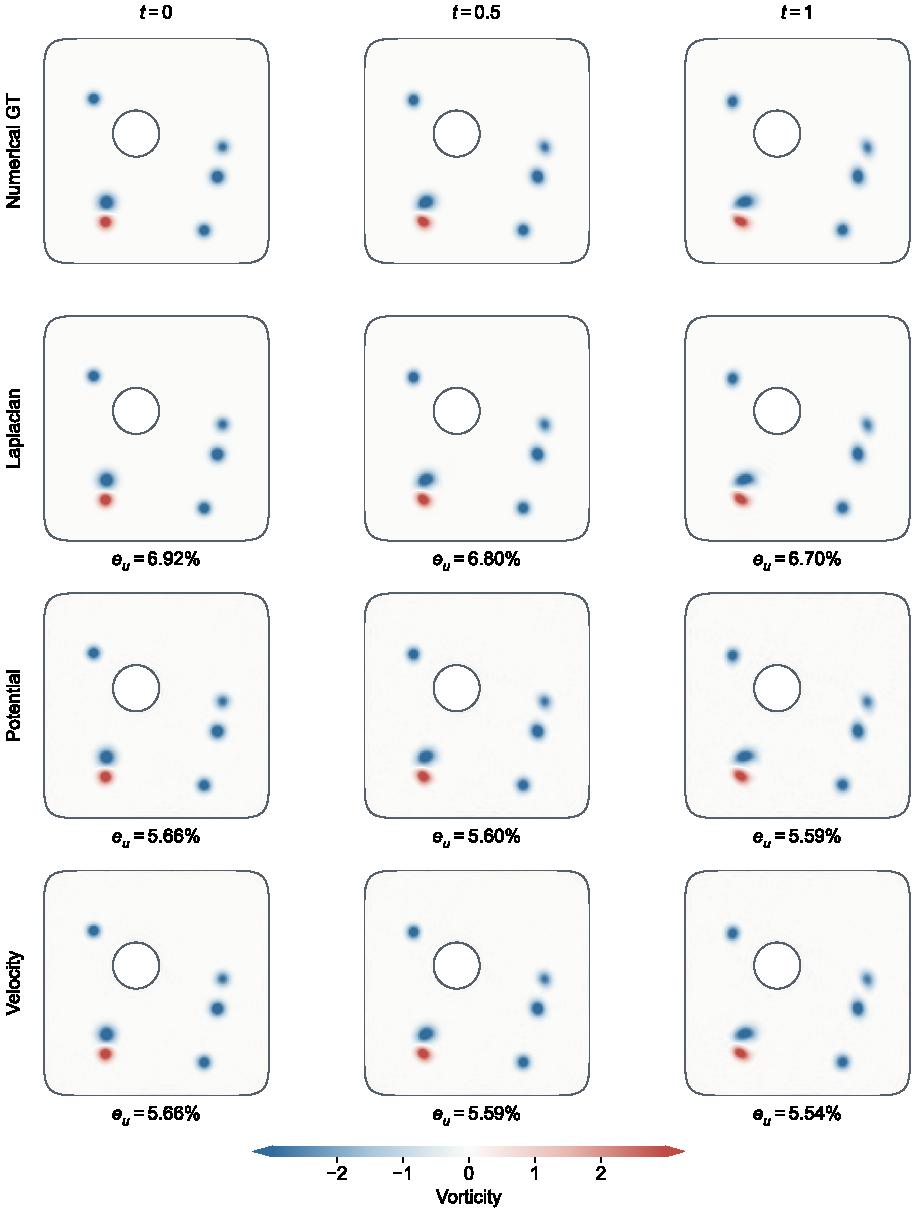
\includegraphics[width=\linewidth,height=.72\textheight,keepaspectratio]{unified_names_20261021_v1/case2_h1_k1024_fourway.pdf}
\caption{\textbf{1-hole planar evolution at $K=1024$.} Rows compare Numerical GT, Laplacian, potential-trained, and velocity-trained bases; columns show $t=0,0.5,1$. Unsmoothed signed vorticity shares a symmetric scale, with colorbar extensions indicating saturation. Annotations give full-domain velocity error for seed 1, state 00 against the common level-2 reference.}
\end{figure}
\begin{figure}[!htb]
\centering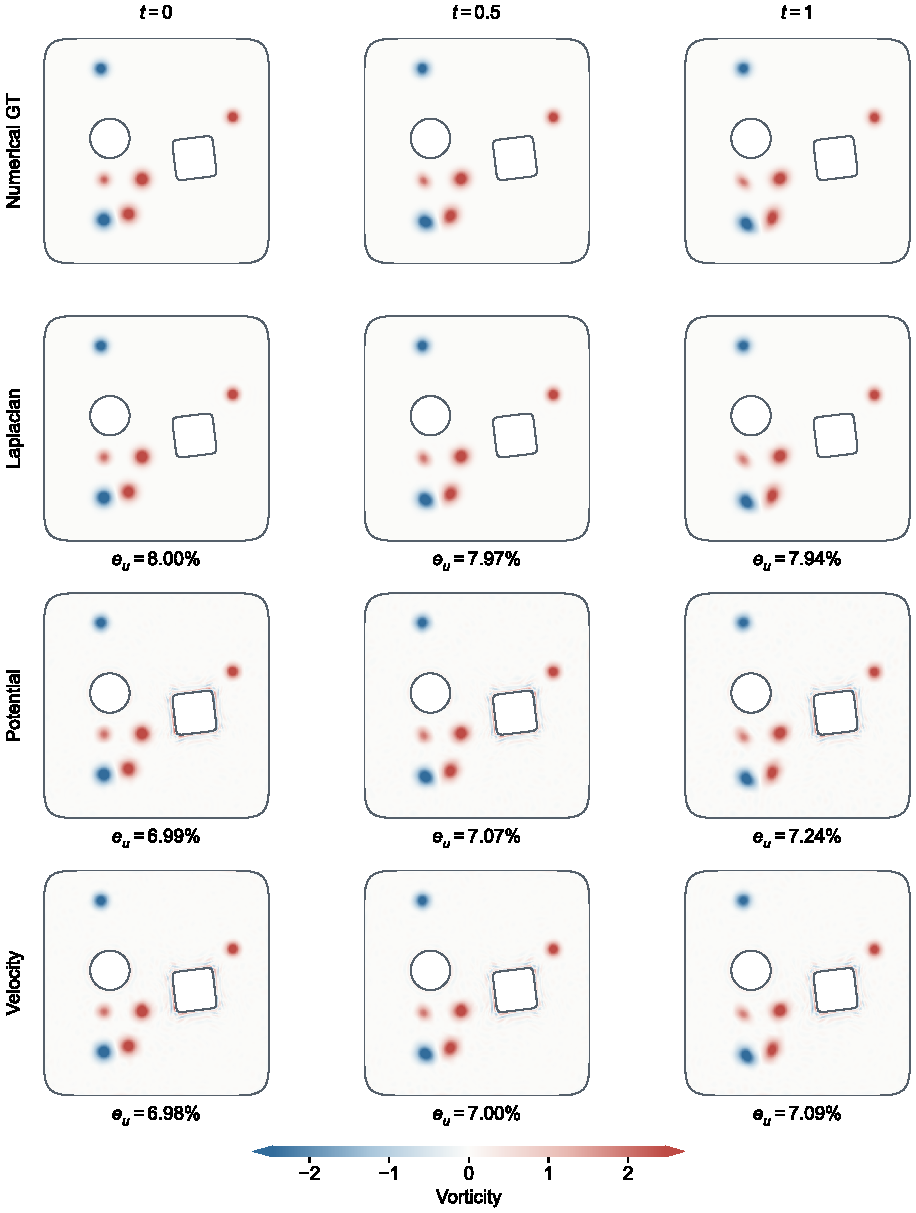
\includegraphics[width=\linewidth,height=.72\textheight,keepaspectratio]{unified_names_20261021_v1/case2_h2_k1024_fourway.pdf}
\caption{\textbf{2-hole planar evolution at $K=1024$.} Rows compare Numerical GT, Laplacian, potential-trained, and velocity-trained bases; columns show $t=0,0.5,1$. Unsmoothed signed vorticity shares a symmetric scale, with colorbar extensions indicating saturation. Annotations give full-domain velocity error for seed 1, state 00 against the common level-2 reference.}
\end{figure}
\begin{figure}[!htb]
\centering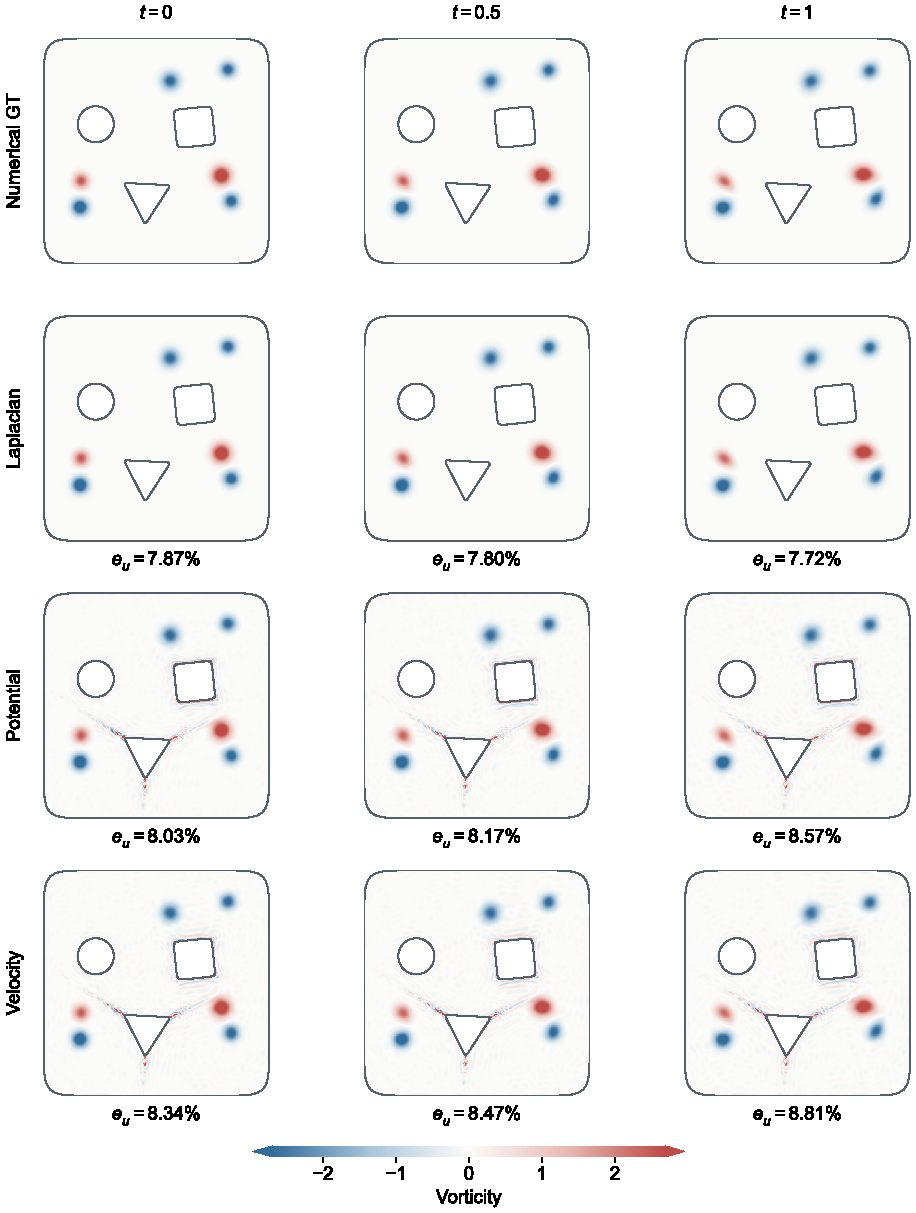
\includegraphics[width=\linewidth,height=.72\textheight,keepaspectratio]{unified_names_20261021_v1/case2_h3_k1024_fourway.pdf}
\caption{\textbf{3-hole planar evolution at $K=1024$.} Rows compare Numerical GT, Laplacian, potential-trained, and velocity-trained bases; columns show $t=0,0.5,1$. Unsmoothed signed vorticity shares a symmetric scale, with colorbar extensions indicating saturation. Annotations give full-domain velocity error for seed 1, state 00 against the common level-2 reference.}
\end{figure}

\section{First eight modes: a basis atlas}
\label{app:modes}
{The periodic and three-dimensional atlases complement the multiply connected comparison in \docref{Figure}{fig:multihole-modes}. Rows identify the construction and columns show its first eight displayed modes, with ordering and representation specified in each caption. Signs and orthogonal rotations within repeated eigenspaces preserve the represented span. Mean-zero scalar displays and per-mode amplitude normalization expose spatial structure while leaving the ROM coordinates unchanged.}
\begin{figure}[!htb]
\centering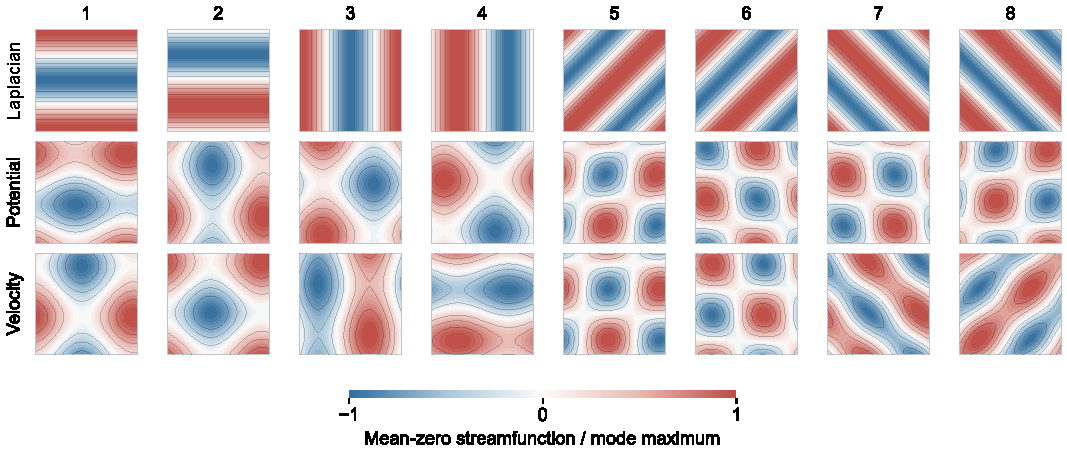
\includegraphics[width=\linewidth,height=.72\textheight,keepaspectratio]{unified_names_20261021_v1/case1_modes.pdf}
\caption{\textbf{First eight periodic modes.} Rows compare analytic Fourier modes and generalized Ritz modes from the potential- and velocity-trained $K=1024$ spans; columns show modes 1--8. Potential Ritz fields use centered potential mass and gradient energy, while velocity Ritz fields use velocity mass and curl energy. Color shows mean-zero streamfunction with per-mode normalization; all 1024 channels contribute to each learned Ritz field.}
\label{fig:modes1}
\end{figure}



\begin{figure}[!htb]
\centering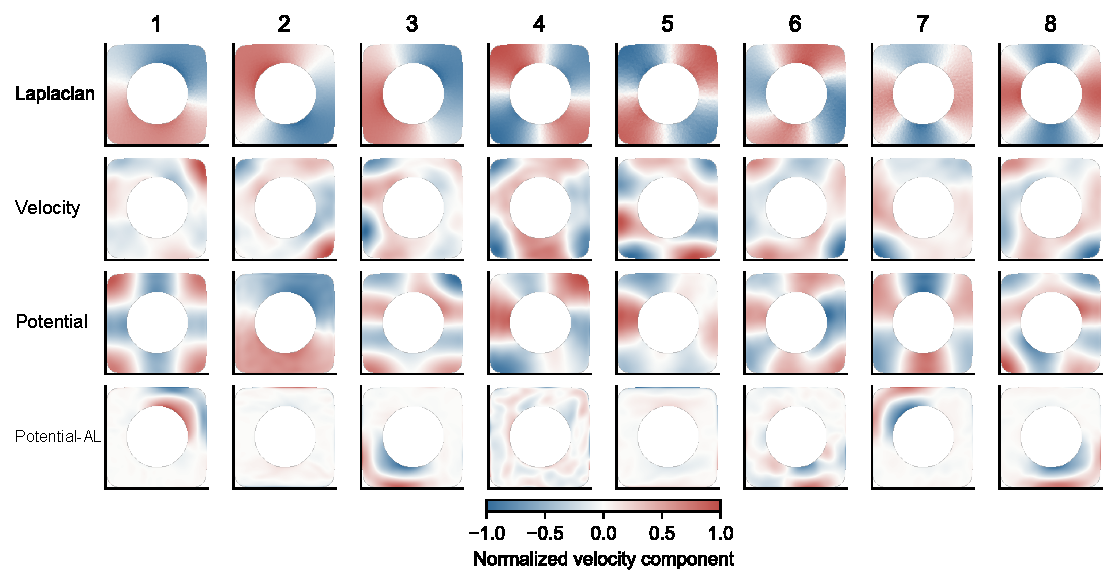
\includegraphics[width=\linewidth,height=.72\textheight,keepaspectratio]{unified_names_20261021_v1/case3_four_method_modes_K32.pdf}
\caption{\textbf{First eight velocity fields at common $K=32$.} Rows compare Laplacian, Velocity, Potential, and Potential-AL; columns show modes 1--8. All methods use the same $z=0.50390625$ slice and per-mode maximum-magnitude normalization of $u_z$. Laplacian fields follow numerical eigenvalue order; learned fields follow their saved channel order, without a display-only Ritz rotation.}
\label{fig:modes3}
\end{figure}
